\documentclass[journal]{IEEEtran}

% *** CITATION PACKAGES ***
%
%\usepackage{cite}
\usepackage{capt-of}%%To get the caption
\usepackage{gensymb}
\usepackage{graphicx} %package to manage images
\graphicspath{ {./images/} }
\usepackage{wrapfig}

\usepackage{amsmath}


\usepackage[style=ieee]{biblatex}
\DeclareLanguageMapping{english}{english-apa}
\addbibresource{references.bib}
\usepackage[justification=centering]{caption}

\usepackage{setspace}

\usepackage{hhline}


\usepackage{changepage} 

\usepackage{booktabs}
\usepackage{xcolor}

\usepackage{makecell}

\renewcommand\theadfont{}

%\raggedbottom

% *** GRAPHICS RELATED PACKAGES ***
%
\ifCLASSINFOpdf
  % \usepackage[pdftex]{graphicx}
  % declare the path(s) where your graphic files are
  % \graphicspath{{../pdf/}{../jpeg/}}
  % and their extensions so you won't have to specify these with
  % every instance of \includegraphics
  % \DeclareGraphicsExtensions{.pdf,.jpeg,.png}
\else
  % or other class option (dvipsone, dvipdf, if not using dvips). graphicx
  % will default to the driver specified in the system graphics.cfg if no
  % driver is specified.
  % \usepackage[dvips]{graphicx}
  % declare the path(s) where your graphic files are
  % \graphicspath{{../eps/}}
  % and their extensions so you won't have to specify these with
  % every instance of \includegraphics
  % \DeclareGraphicsExtensions{.eps}
\fi
% graphicx was written by David Carlisle and Sebastian Rahtz. It is
% required if you want graphics, photos, etc. graphicx.sty is already
% installed on most LaTeX systems. The latest version and documentation
% can be obtained at: 
% http://www.ctan.org/pkg/graphicx
% Another good source of documentation is "Using Imported Graphics in
% LaTeX2e" by Keith Reckdahl which can be found at:
% http://www.ctan.org/pkg/epslatex
%
% latex, and pdflatex in dvi mode, support graphics in encapsulated
% postscript (.eps) format. pdflatex in pdf mode supports graphics
% in .pdf, .jpeg, .png and .mps (metapost) formats. Users should ensure
% that all non-photo figures use a vector format (.eps, .pdf, .mps) and
% not a bitmapped formats (.jpeg, .png). The IEEE frowns on bitmapped formats
% which can result in "jaggedy"/blurry rendering of lines and letters as
% well as large increases in file sizes.
%
% You can find documentation about the pdfTeX application at:
% http://www.tug.org/applications/pdftex

\begin{document}

\begin{titlepage}
    {\centering
        \vspace*{20em}
        {
        \huge 
        \begin{spacing}{1.5}
            Lab Report \#3: LT Spice Simulation of Polyphase Circuits 
            \\
            Advanced Circuits Lab (ENGR$-$UH 2311),\\
            Spring 2019
            \bigskip
            \Large
            \\
            Polyphase circuits in LTSPice
  
            \\
            \bigskip
            Deadline: May 1, 2019 
        \end{spacing}

        }
        
    }
    \vfill
    
    {
    \large
    
    \begin{spacing}{1.5}
    \noindent Barkin Simsek, {\it {bs3528@nyu.edu}} 
    \\
    Nishant Aswani, {\it {nsa325@nyu.edu}}
    \\
    Section \#1% <-this % stops a space
    \\
    Workstation \#8% <-this % stops a space
    \end{spacing}
    }


\end{titlepage}
\pagenumbering{gobble}
%\clearpage\mbox{} % adds and empty page
%\clearpage
\pagenumbering{arabic}
\setcounter{page}{1}

%\title{Demonstration of a Voltage Divider With A Variable Resistor}

%\author{Barkin Simsek,~\IEEEmembership{bs3528@nyu.edu};
%Nishant Aswani,~\IEEEmembership{nsa325@nyu.edu}
%\\ Table Number: \#}% <-this % stops a space


% The paper headers
\markboth{Simsek, Aswani, Advanced Circuits Lab 2019}%
{}

% make the title area
%\maketitle

% As a general rule, do not put math, special symbols or citations
% in the abstract or keywords.
\begin{abstract}
In this lab, the purpose was using the LTSpice software to simulate a wye-wye circuit and measure different properties such as voltages, currents, instantaneous power dissipated, and the average power dissipated at different points of the circuit.

\end{abstract}

%%%%%%%%%%%%%%%%%%
%% Introduction %%
%%%%%%%%%%%%%%%%%%
\section{Introduction}

\IEEEPARstart{W}\lowercase{hen} referring to transformer load configurations, the two options are wye-connected and  delta-connected configurations (see Figures \ref{fig:wyeconfig} and \ref{fig:deltaconfig}).

\begingroup
    \centering
    \medskip
    %width=\columnwidth
    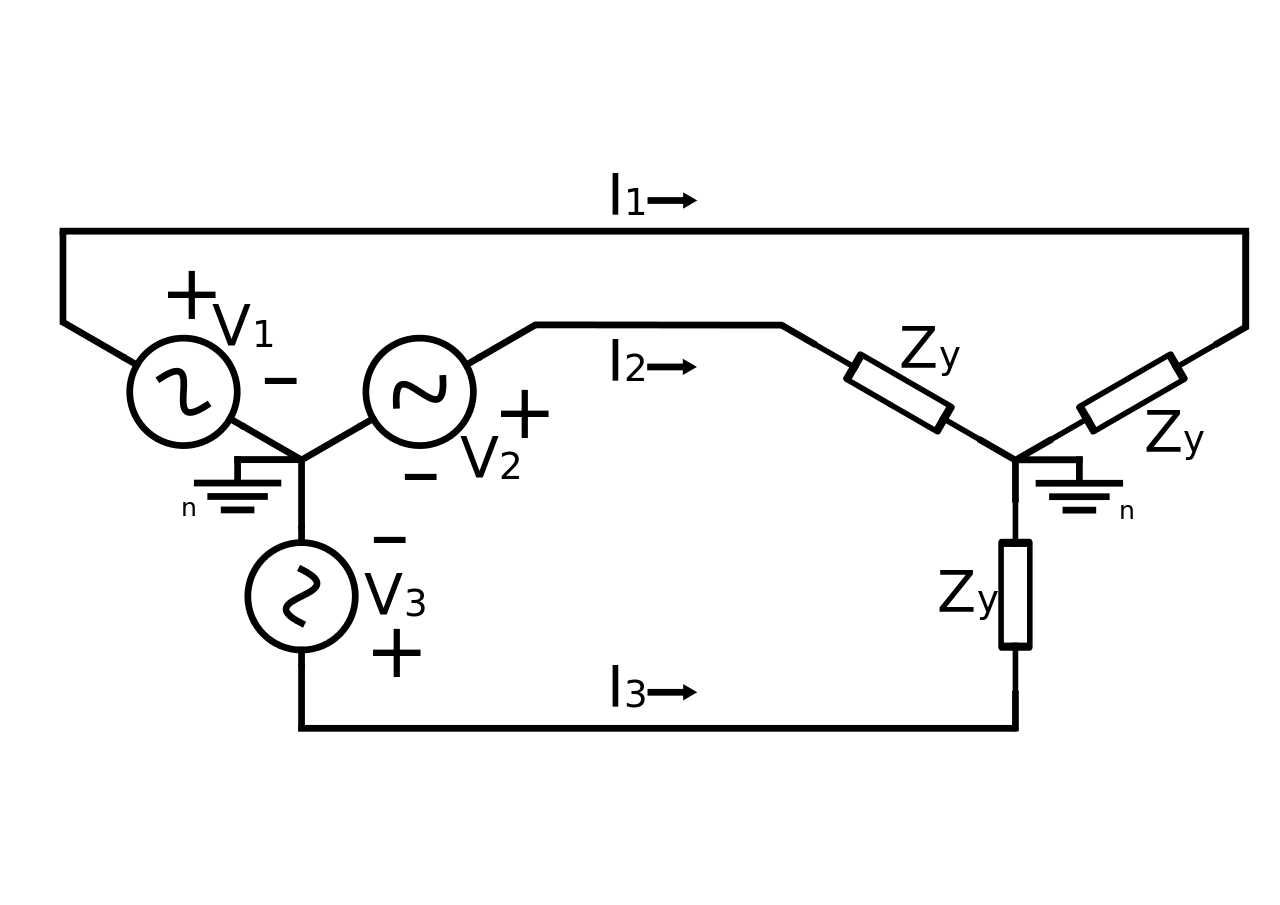
\includegraphics[width=\columnwidth]{images/lab9_3.png}
    \captionof{figure}{A three-phase AC wye-connected source to a wye-connected load}
    \label{fig:wyeconfig}
\endgroup


\begingroup
    \centering
    \medskip
    %width=\columnwidth
    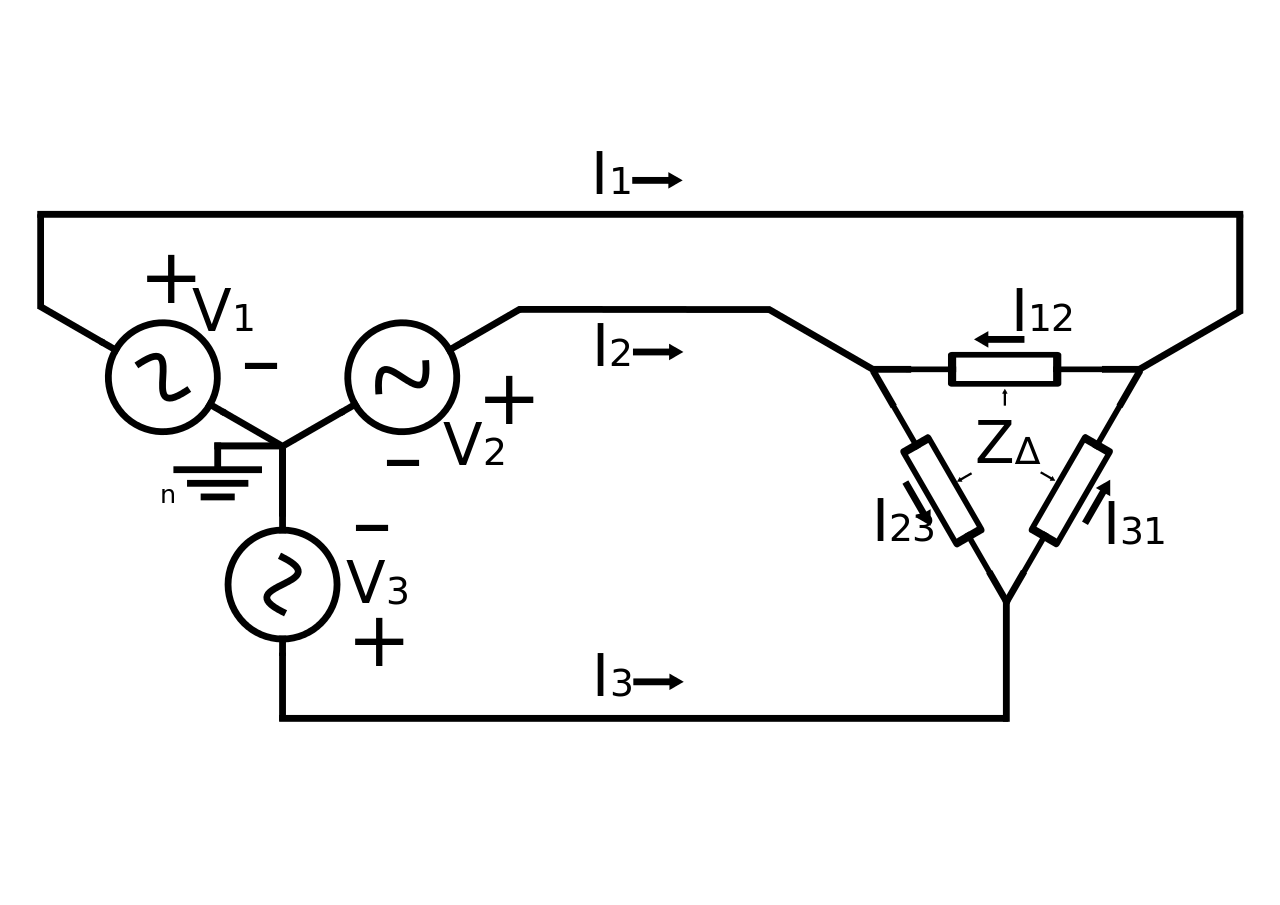
\includegraphics[width=\columnwidth]{images/lab9_4.png}
    \captionof{figure}{A three-phase AC wye-connected source to a delta-connected load}
    \label{fig:deltaconfig}
\endgroup

\noindent In the wye configuration, the phase voltage, voltage across the total load in one phase, is a factor of $\sqrt{3}$ smaller than the line voltage, the voltage between source lines, but the line and phase currents are equivalent. On the other hand, in a delta configuration, the phase and line voltages are equivalent, but the phase current is smaller by a factor of $\sqrt{3}$ than the line current. These relations are summarized with equations \ref{eq:configrelationswye} and \ref{eq:configrelationsdelta}. 

For wye configurations:

\begin{equation}
    \begin{split}
        V_{line} & = \sqrt{3} \times {V_{phase}}\\
        I_{line} & = I_{phase}\\
    \end{split}
    \label{eq:configrelationswye}
\end{equation}


For delta configurations:  
\begin{equation}
    \begin{split}
        V_{line} & = V_{phase}\\
        I_{line} & = \sqrt{3}\times{I_{phase}}\\
    \end{split}
    \label{eq:configrelationsdelta}
\end{equation} 

\noindent The wye-connection provides three-phases and four wires, allowing for there to be flexibility in how the loads are connected: a load may be connected using a single phase or all three phases. This flexibility is not provided in delta-connected loads. Also, it difficult to guarantee a balanced load distribution in real life application. Therefore, wye-connection is considered to be practical while delta-connection is not considered as a practical connection type.\\

\noindent However, delta-connections are superior to wye-connections at fault tolerance. In the case of a "delta-delta" connection, where line voltage is equivalent to phase voltage, if one of the three sources were to fail, there would be no effect on the voltages across the loads. The only effect would be an increased phase current. Considering a "wye-delta" configuration, a failed winding on one of the sources would decrease the voltage across two of the three loads. Finally, looking at a "wye-wye" configuration, a failed source would cause decrease in performance for two of the loads and completely lose one load. In all of the scenarios, a delta connection provides a better hedge against faults.\\ 

\noindent The following experiment examined a wye-wye configuration, which has the benefit of common neutral connections that can be grounded.


%%%%%%%%%%%%%%%%%%%%%%%%%
%% Experimental Set-up %%
%%%%%%%%%%%%%%%%%%%%%%%%%
\section{Experimental Set-up}

\noindent The LTSpice software (Windows XP edition) by Analog Devices, Inc. was used to use construct circuits shown in Figures \ref{fig:ac1} and \ref{fig:ac2}. These circuits were constructed in two separate files. The simulation feature of LTSpice was used to plot the voltages, currents, and instantaneous power dissipated, as well as determine the average power dissipated at different points of the circuit.

\begingroup
    \centering
    \medskip
    %width=\columnwidth
    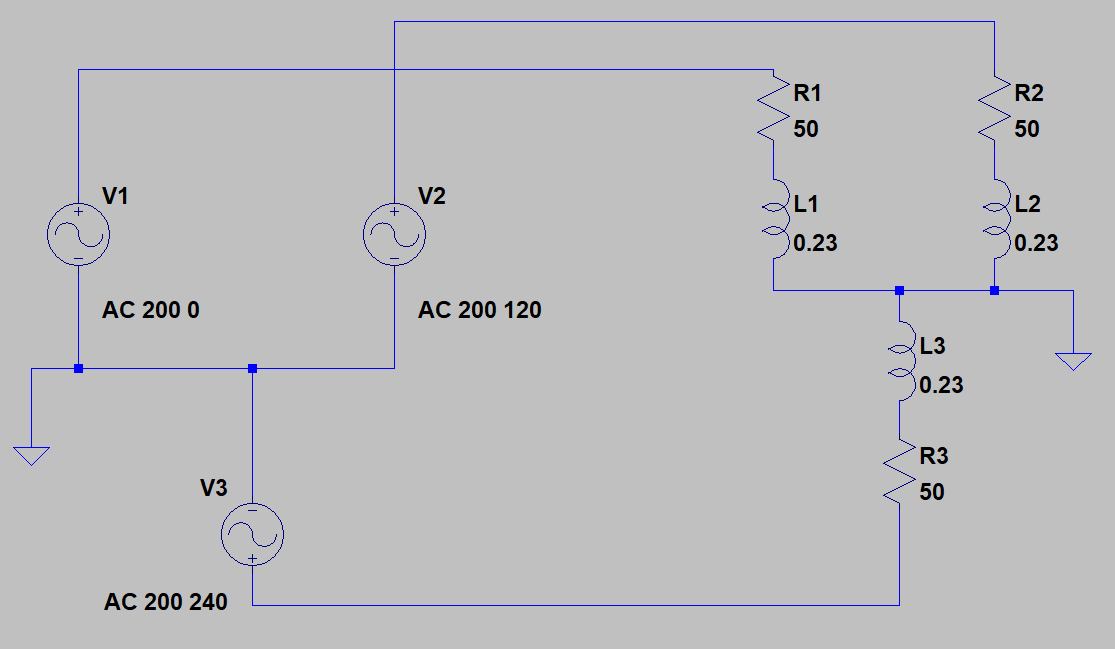
\includegraphics[width=\columnwidth]{images/lab9_2.png}
    \captionof{figure}{A balanced wye-wye connection with LT Spice's AC signal generator}
    \label{fig:ac1}
    \medskip
\endgroup

\begingroup
    \centering
    \medskip
    %width=\columnwidth
    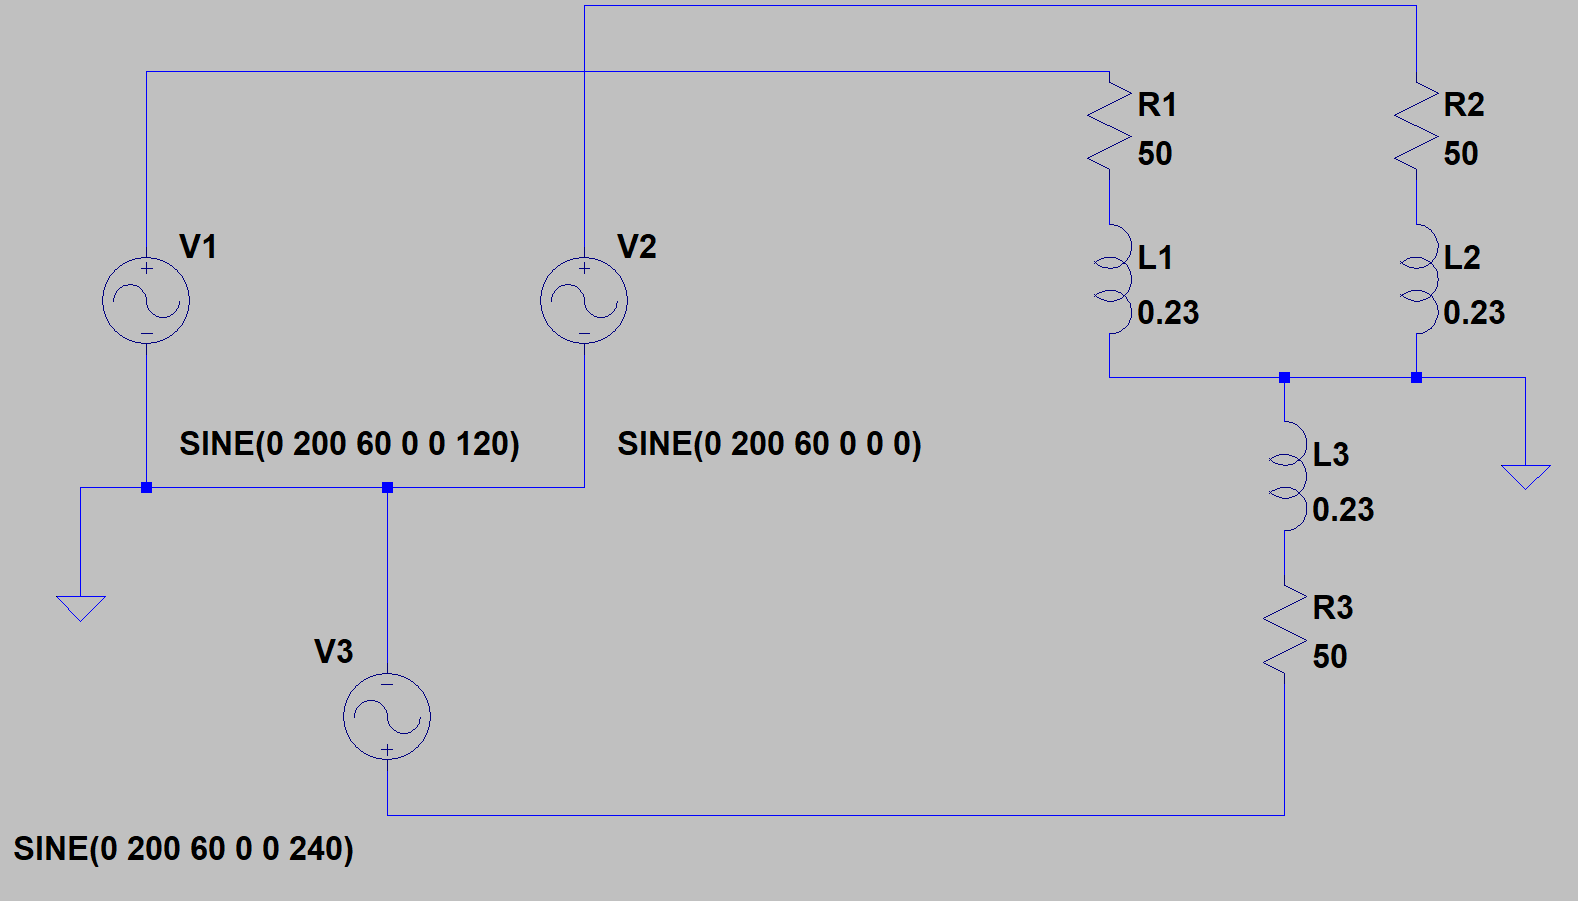
\includegraphics[width=\columnwidth]{images/lab9_1.png}
    \captionof{figure}{A balanced wye-wye connection with LT Spice's sine wave generator}
    \label{fig:ac2}
    \medskip
\endgroup

\\

\noindent In the experiment, three 0.23$H$ inductors, three $50\ohm$ resistors, and three AC voltage sources were used. With a balanced load of one inductor and one resistor on each phase, AC voltage sources were altered to supply signals with phase shifts, such as AC 200V with 0\degree, 120\degree, and 240\degree. Similarly, in the second circuit, sine waves were supplied with an amplitude of 200V and phase differences of 0\degree, 120\degree, and 240\degree. All components were connected with appropriate nets as specified in the circuit diagrams and results of the simulated cases were recorded.

%%%%%%%%%%%%%%%%%%%%%%%%%%%%
%% Results and Discussion %%
%%%%%%%%%%%%%%%%%%%%%%%%%%%%
\section{Results and Discussion}

\noindent All configurations were simulated successfully in the LTSpice software. Graphs of different measurements are shared below:


\subsection{Phase and Line Voltage}

\noindent In the case of polyphase systems, each voltage source provides a certain voltage phase shifted from the other sources. As a result, the load, say a motor, receives a kick more frequently and thus operates smoothly when compared to a single phase power source, as shown in Figure \ref{fig:motor}.\\

\begingroup
    \centering
    \medskip
    %width=\columnwidth
    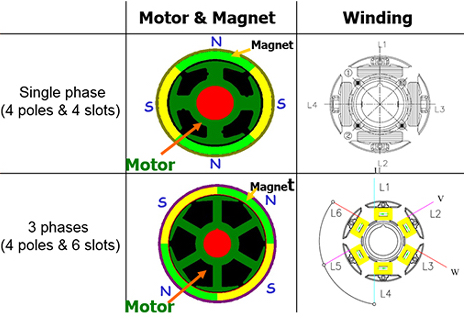
\includegraphics[width=\columnwidth]{images/motor.jpg}
    \captionof{figure}{The differences in the way single phase and three phase motors are structures \cite{motor}}
    \label{fig:motor}
    \medskip
\endgroup


\noindent A 0.23 H inductor has an impedance of $86.6j$ at a frequency of 60Hz. Equations \ref{eq:calc1} and  \ref{eq:calc2} shows the calculated phase/line current, which is multiplied by the impedance of the inductor to determine the voltage across the inductor. 

%%%%%%%%%% %%%%%%%%%%%%%%%%%%%%%%%%%


\begin{equation}
I_{line} = I_{phase} = \frac{200}{50+86.6j} = 2 \angle -59.99\degree
\label{eq:calc1}
\end{equation}


\begin{equation}
V_{inductor} = (2 \angle -59.99\degree)(86.6j) = 173.2 \angle 30.01\degree
\label{eq:calc2}
\end{equation}


%%%%%%%%%%%%%%%%%%%%%%%%%%%%%%%%%%%%%%

\noindent Figure \ref{fig:load_freq_volt} shows a plot of frequency against voltage across the inductor in each phase. Referring back to equation \ref{eq:calc2}, we see that the voltage across the inductor is approximately 173 V at 60 Hz. Looking at the far right of the graph below confirms this result, as the rising red trace shows a voltage of approximately 170V at 60 Hz. The green trace also confirms the calculated result, as the phase is 30\degree at around 60 Hz. The graph also shows the general relation that as frequency increases, the voltage across the inductor increases, while the phase shift decreases.

\begingroup
    \centering
    \medskip
    %width=\columnwidth
    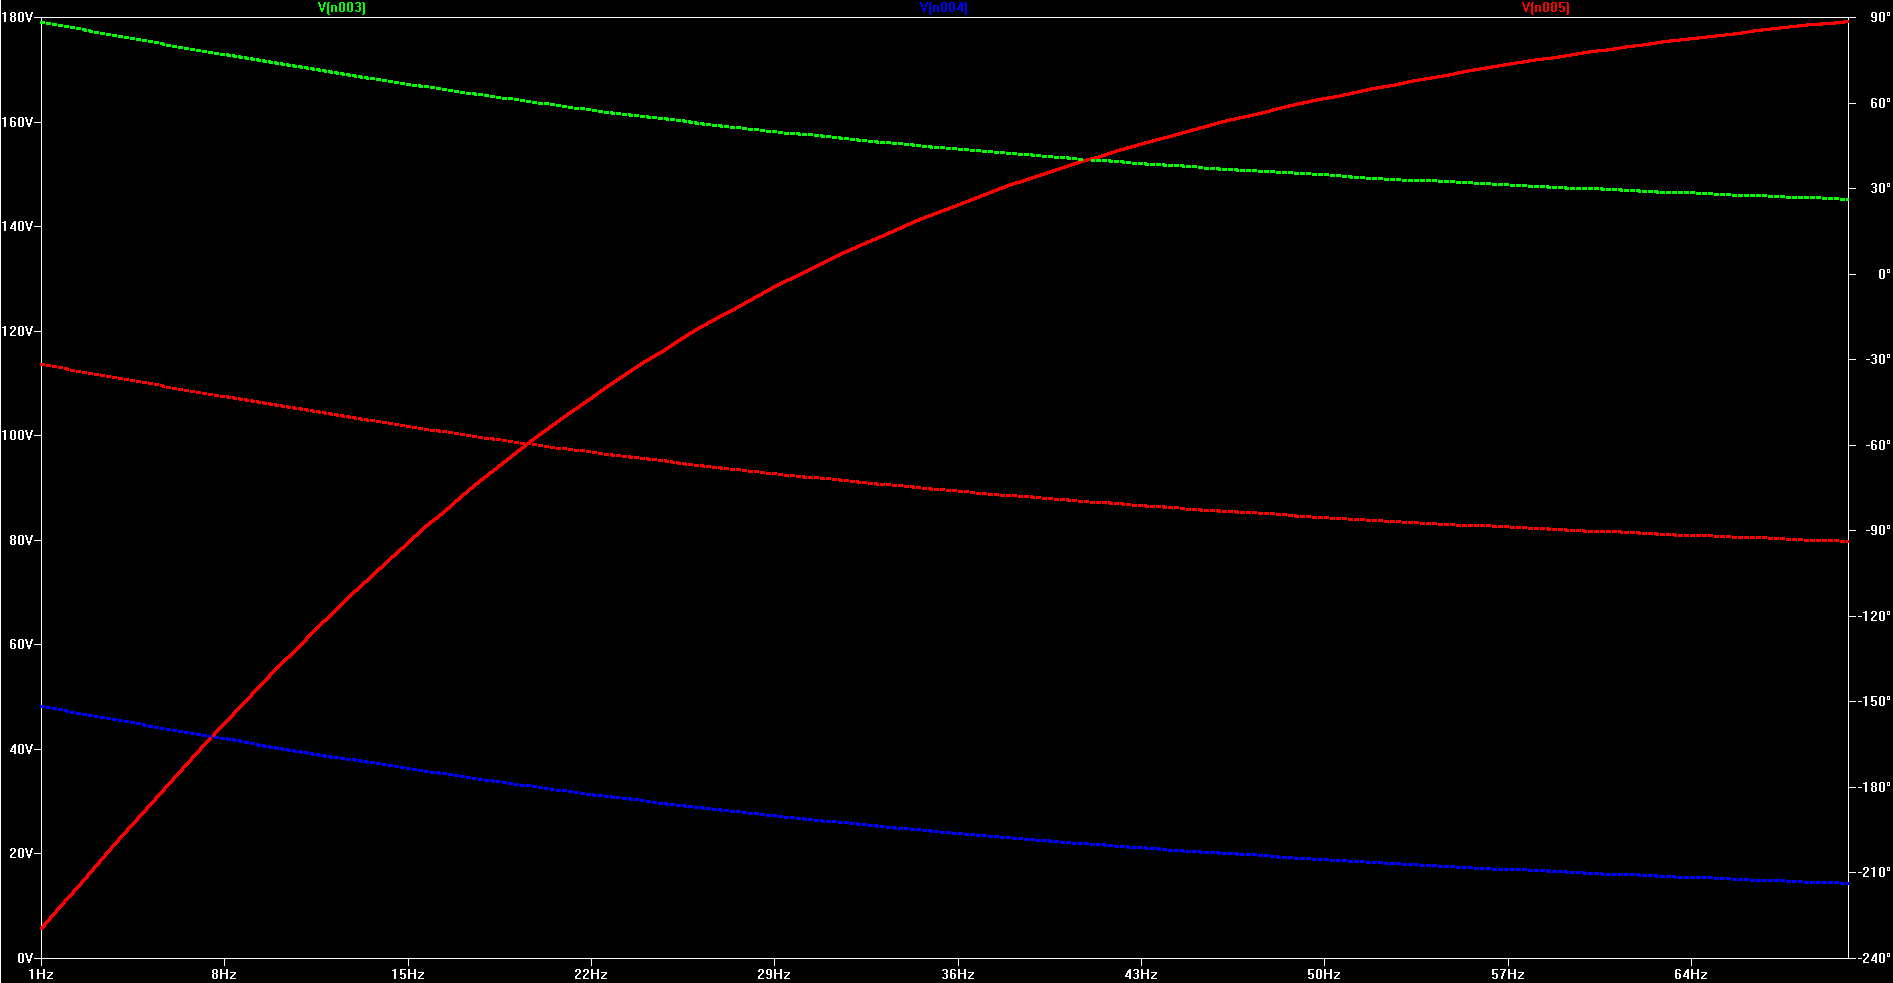
\includegraphics[width=\columnwidth]{images/Lab_9_ss_1.PNG}
    \captionof{figure}{Voltage across the inductor plotted against frequency}
    \label{fig:load_freq_volt}
    \medskip
\endgroup


\noindent Providing a sine wave to the circuit and plotting the voltage versus time, Figures \ref{fig:load_time_volt} and \ref{fig:source_time_volt} show the voltage across the inductor and the entire load.

\begingroup
    \centering
    \medskip
    %width=\columnwidth
    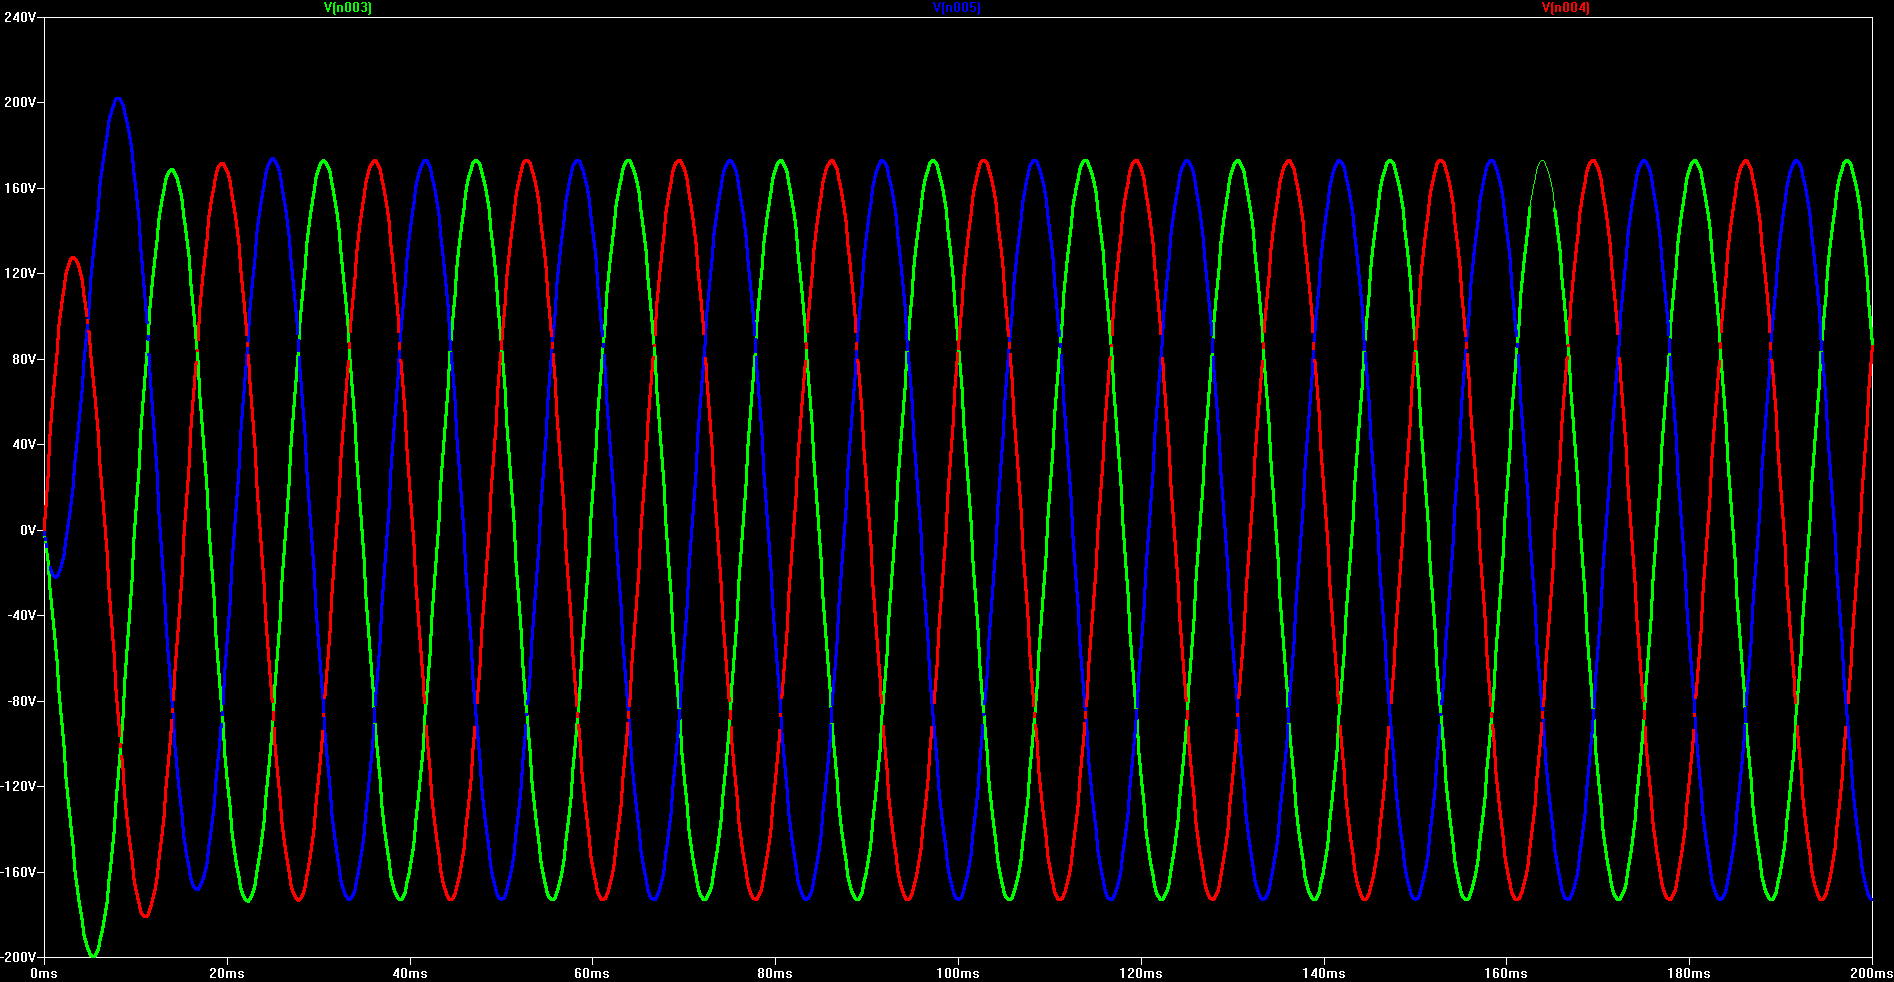
\includegraphics[width=\columnwidth]{images/Lab_9_ss_5.PNG}
    \captionof{figure}{Voltage across the inductor plotted against time}
    \label{fig:load_time_volt}
    \medskip
\endgroup



\begingroup
    \centering
    \medskip
    %width=\columnwidth
    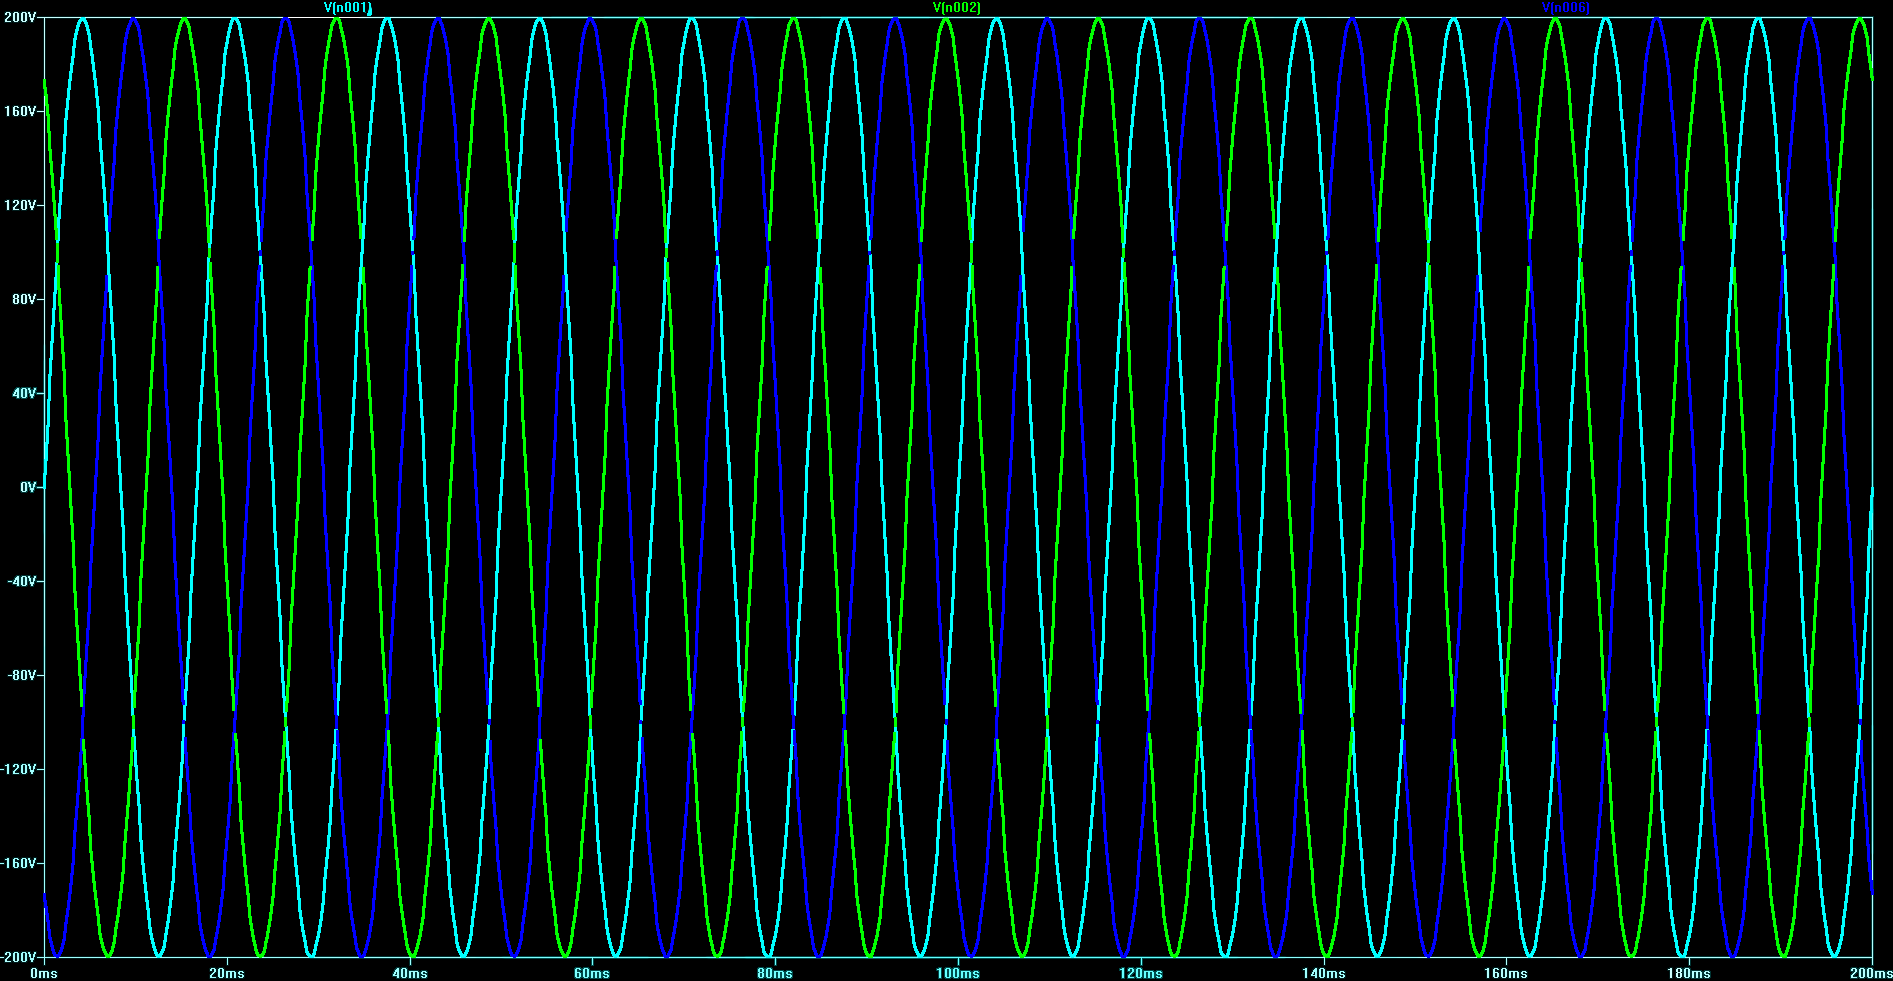
\includegraphics[width=\columnwidth]{images/Lab_9_ss_6.PNG}
    \captionof{figure}{Voltage across the total load against time}
    \label{fig:source_time_volt}
    \medskip
\endgroup

\noindent In the above cases, the voltage oscillates, peaking at approximately 170V across the inductor in Figure \ref{fig:load_time_volt}. Given that the sine wave was provided at a frequency of 60 Hz, this confirms the calculations in equations \ref{eq:calc1} and  \ref{eq:calc2}. \\

\noindent In the case of wye-wye configurations, it is known that the line voltage is not equivalent to the phase voltage. More specifically, the line voltage is greater by a factor of $\sqrt{3}$. Therefore, one would expect that the line voltage, in this case, would be $\sqrt{3}\cdot 200 = 346.41$. Figure \ref{fig:line_voltage} plots the line voltage between $V_{1}$ and $V_{2}$ across time, peaking at approximately 350V,  thus confirming the expected value. \\

\begingroup
    \centering
    \medskip
    %width=\columnwidth
    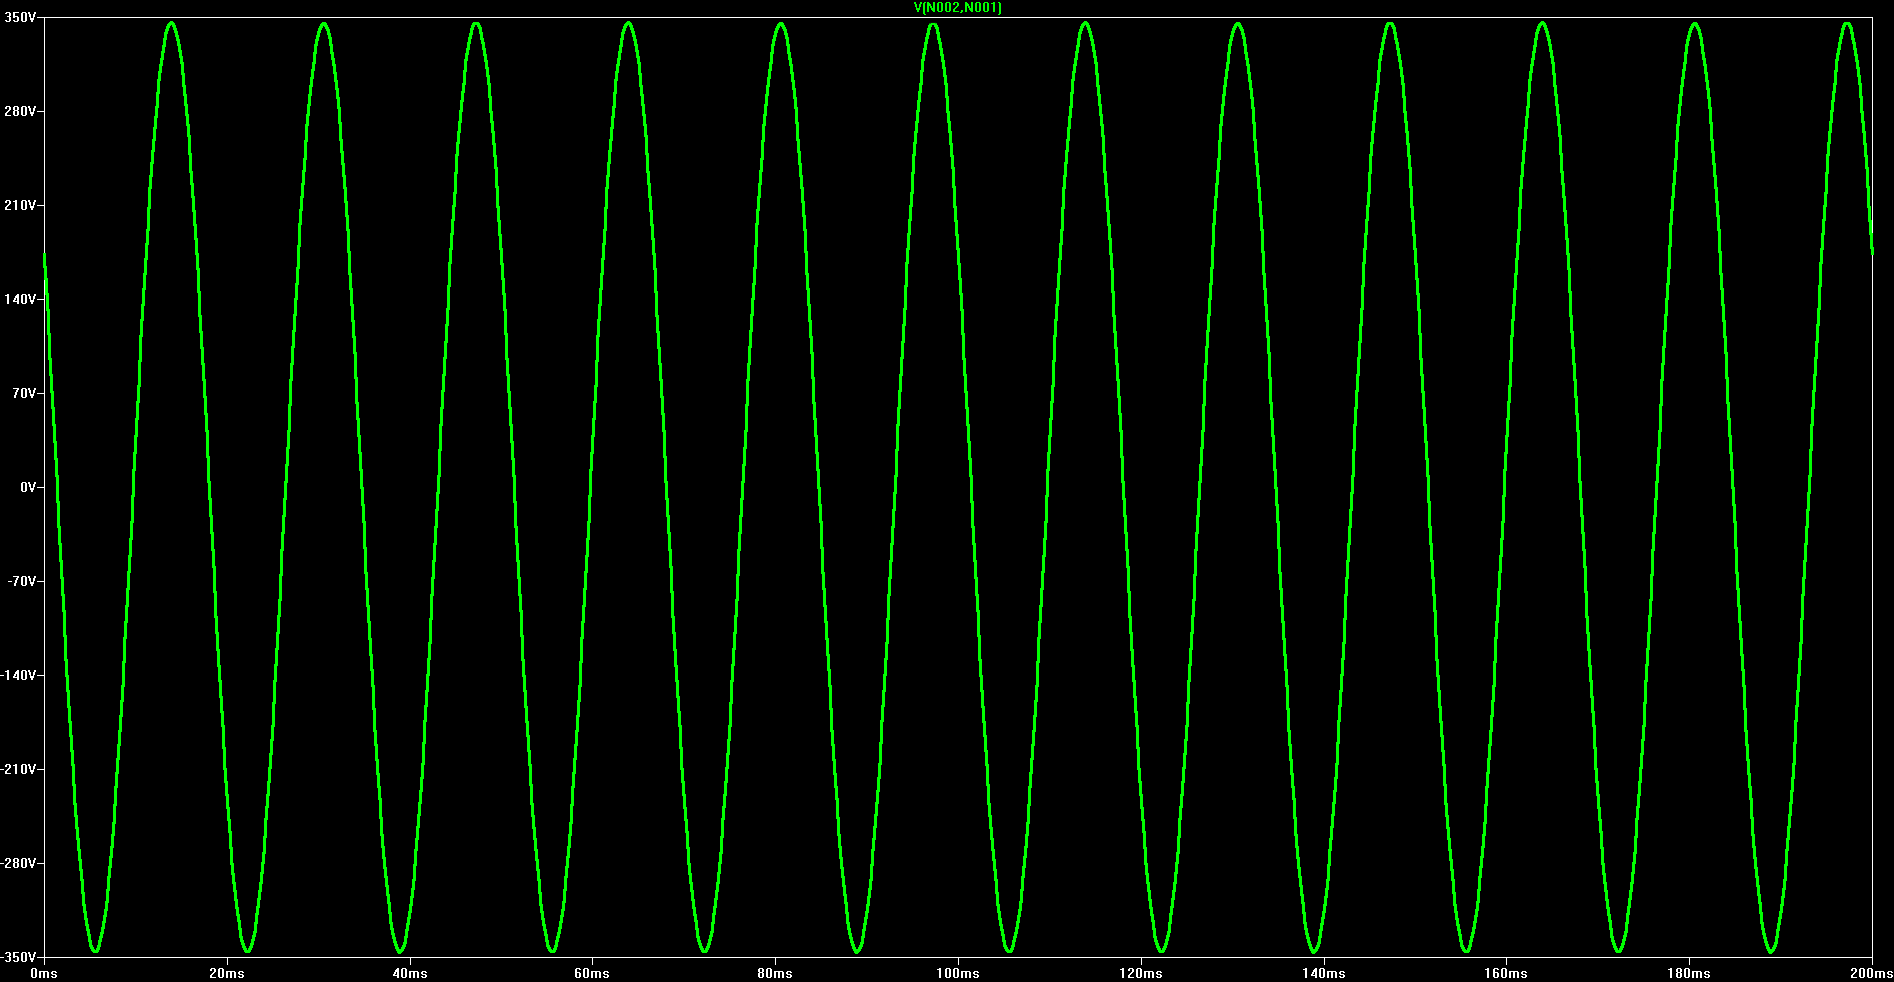
\includegraphics[width=\columnwidth]{images/Lab_9_ss_10.PNG}
    \captionof{figure}{  line voltage between V1 and V2}
    \label{fig:line_voltage}
    \medskip
\endgroup



%%%%%%%%%%%%%%%%%%%%%%%%%%%%%%%%%%%%%%%%%%%%%%%%%%%%%%%%%%%%%%%%%%%%%
\subsection{Phase and Line Current}
%%%%%%%%%%%%%%%%%%%%%%%%%%%%%%%%%%%%%%%%%%%%%%%%%%%%%%%%%%%%%%%%%%%%%

\noindent The following plots (Figures \ref{fig:current_resistor}, \ref{fig:current_inductor}, and \ref{fig:current_power_source}) depict the current across the resistor, inductor, and power source. As expected, all the currents are equivalent, because wye-wye configurations ensure equivalent phase and line currents. Furthermore, it is clear that at a higher frequency, the current decreases. This is explained by the tendency of the inductor to have a high impedance at high frequencies. Using Ohm's law shows that a high impedance across a given voltage, decreases the current across the load. \\

\noindent The figures also confirm the expected amperage value. All the graphs show a current of approximately 2A at a frequency of 60Hz, which is the calculated value from equation \ref{eq:calc1}. If we assume the light blue trace to represent the current at $V_{1}$, we also see the expected phase shift of -60\degree at 60Hz. \\

\begingroup
    \centering
    \medskip
    %width=\columnwidth
    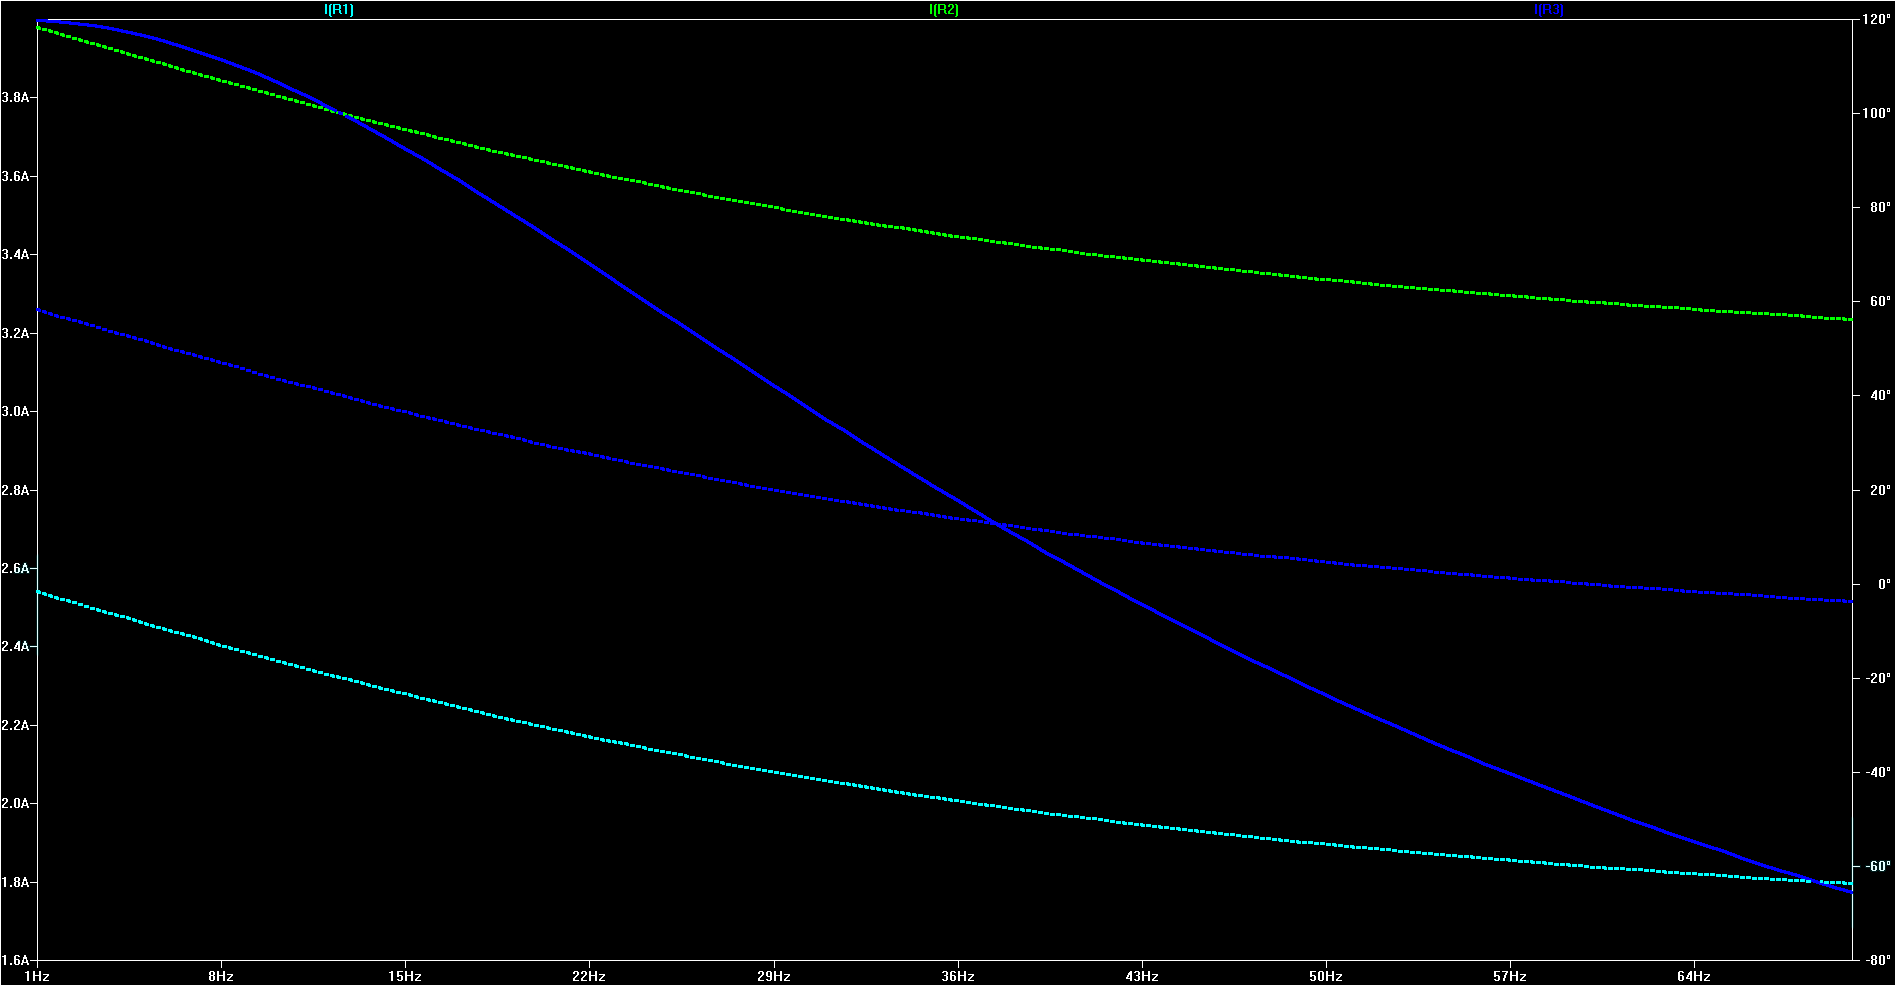
\includegraphics[width=\columnwidth]{images/Lab_9_ss_2.PNG}
    \captionof{figure}{Current across the resistor}
    \label{fig:current_resistor}
    \medskip
\endgroup


\begingroup
    \centering
    \medskip
    %width=\columnwidth
    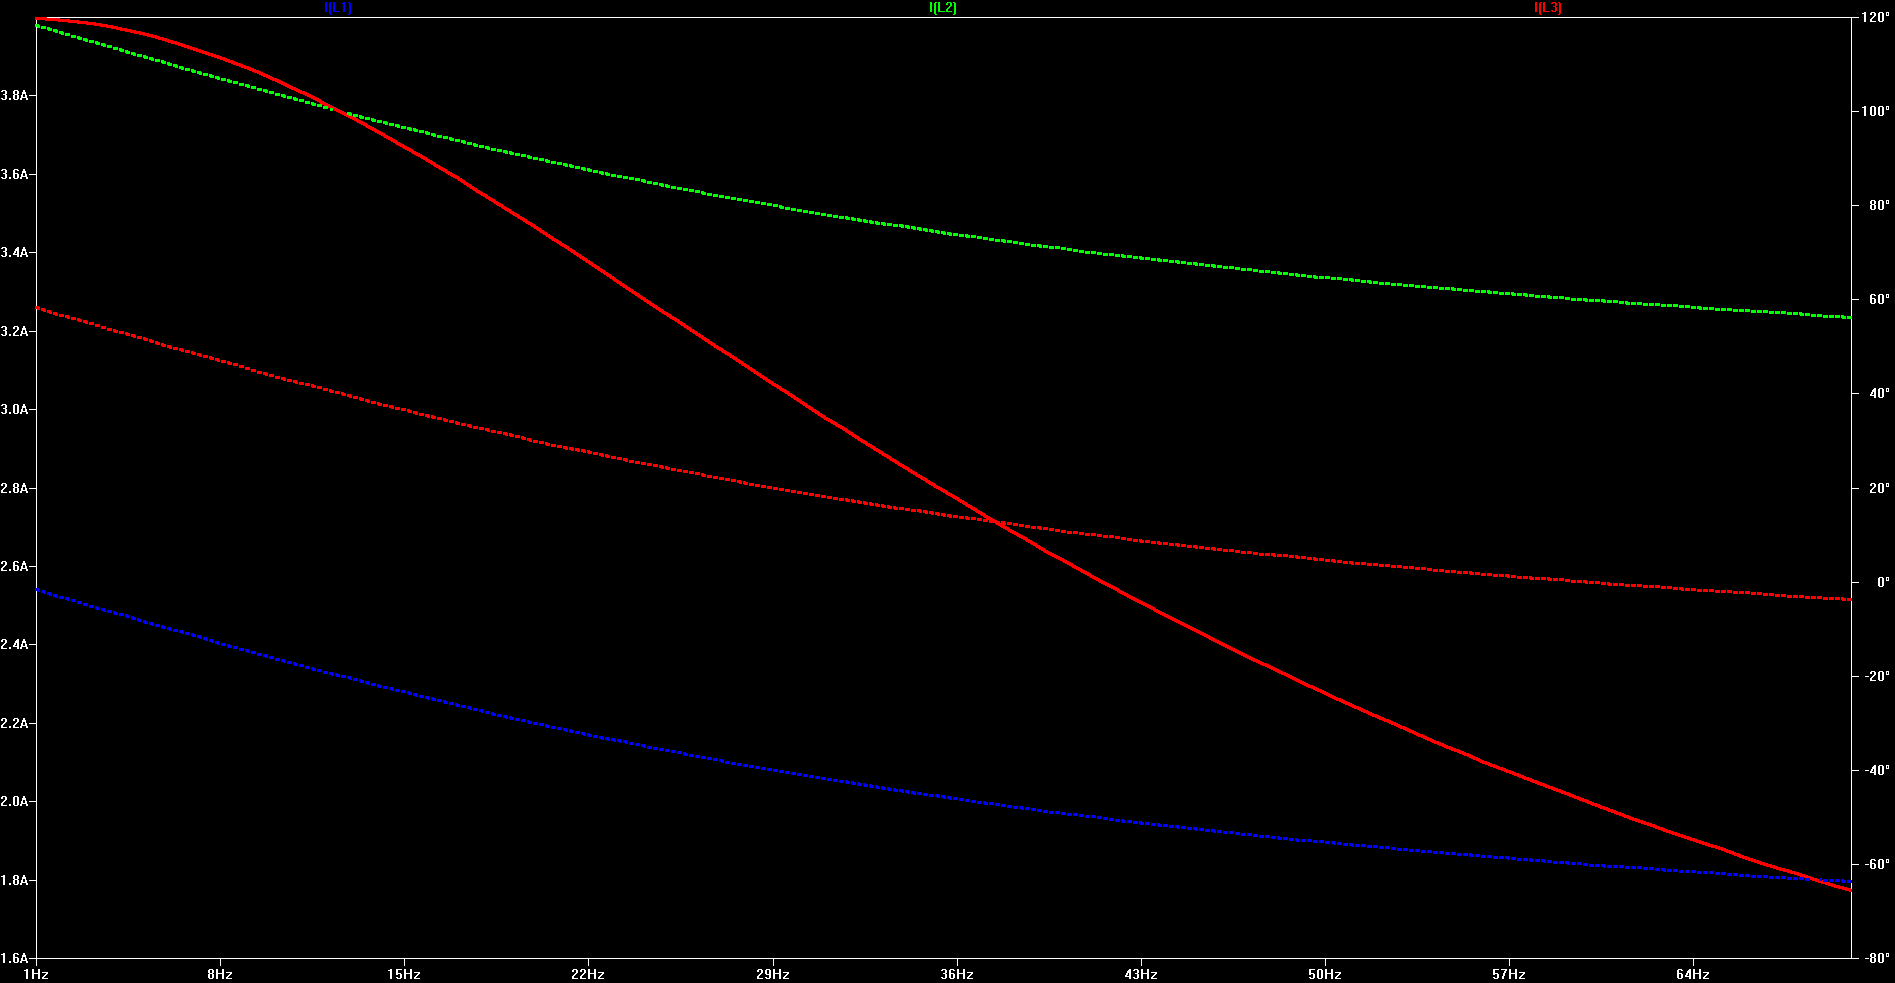
\includegraphics[width=\columnwidth]{images/Lab_9_ss_3.PNG}
    \captionof{figure}{Current across the inductor}
    \label{fig:current_inductor}
    \medskip
\endgroup


\begingroup
    \centering
    \medskip
    %width=\columnwidth
    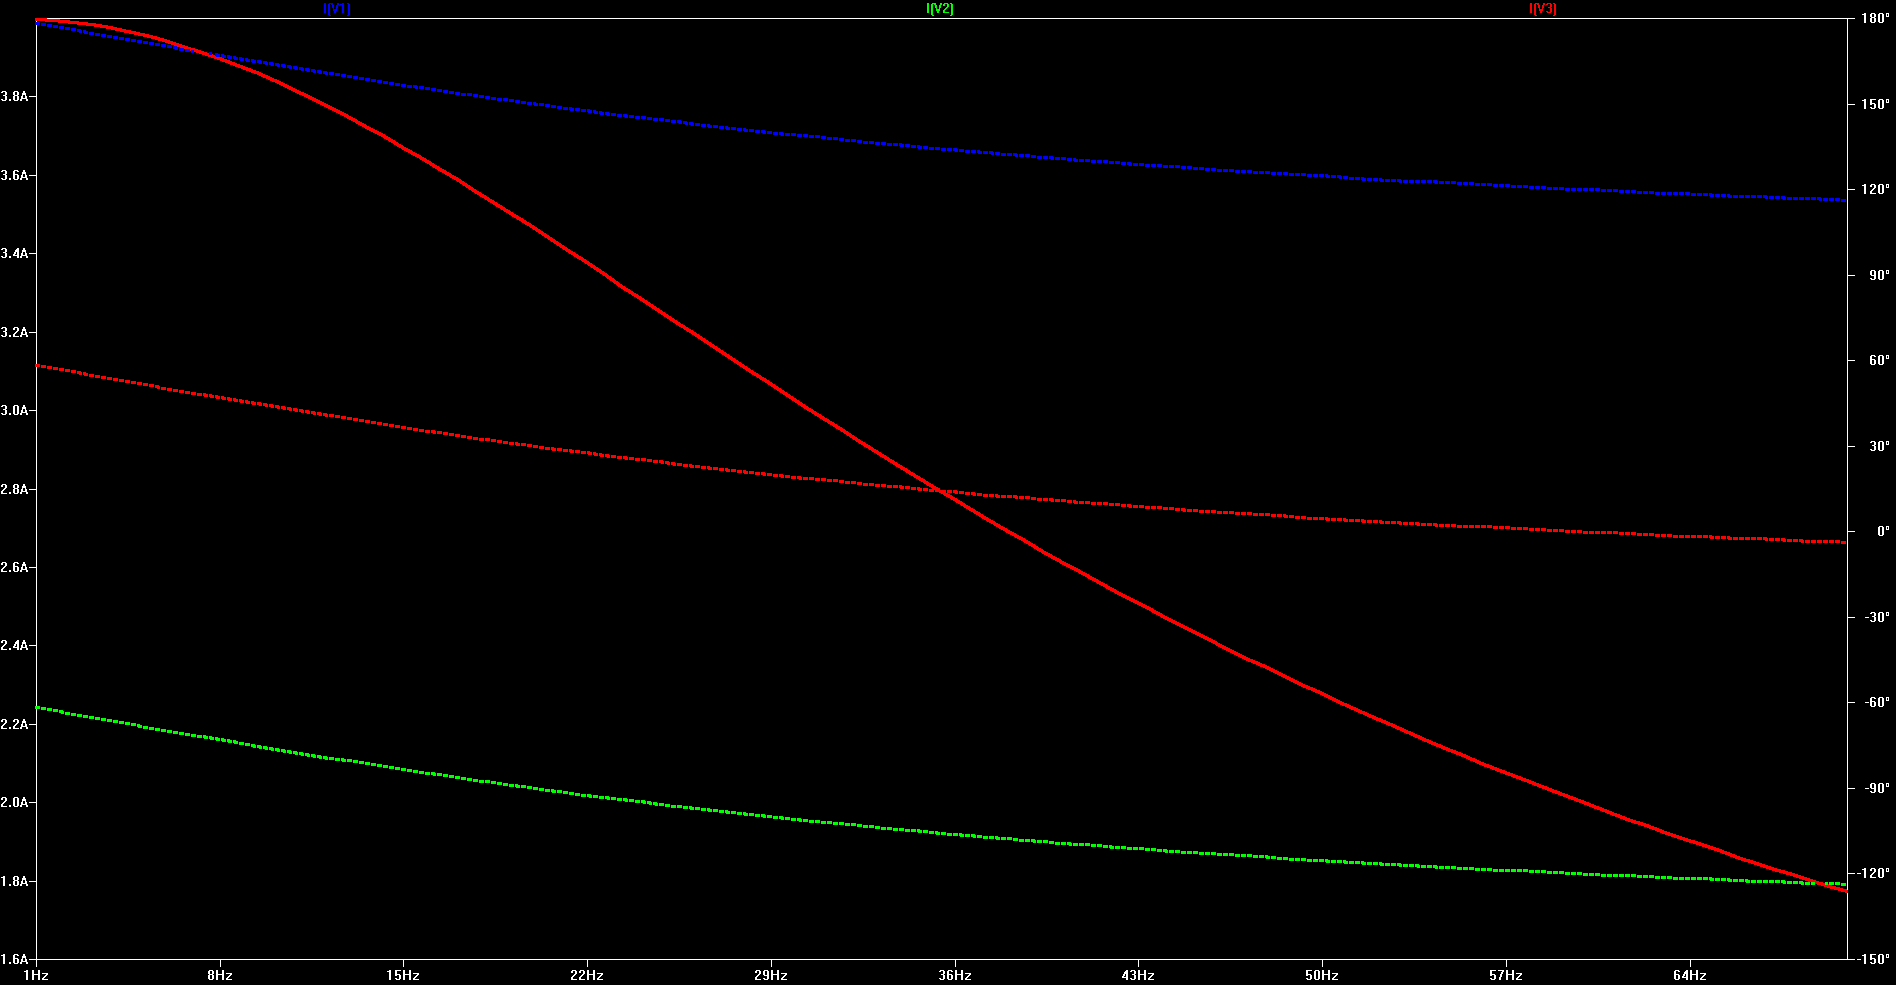
\includegraphics[width=\columnwidth]{images/Lab_9_ss_4.PNG}
    \captionof{figure}{Current across the power source}
    \label{fig:current_power_source}
    \medskip
\endgroup

%%%%%%%%%%%%%%%%%%%%%%%%%%%%%%%%%%%%%%%%%%%%%%%%%%%%%%%%%%%%%%%%%%%%%
\subsection{Instantaneous and Average Power}
%%%%%%%%%%%%%%%%%%%%%%%%%%%%%%%%%%%%%%%%%%%%%%%%%%%%%%%%%%%%%%%%%%%%%
\noindent Instantaneous power is the power across any component at any instant of time. The equation below calculates the apparent power through the inductor. 

\begin{equation} 
I^2 \cdot Z_{Inductor} = ({2.00 \angle -59.99})^2 \cdot 86.6j = 346.42 \angle -29.99 VAR
\label{eq:calc3}
\end{equation}

\noindent Figure \ref{fig:inst_power_inductor} shows a peak to a peak power of approximately 340W. Comparing this result to equation \ref{eq:calc3} confirms the expected magnitude of the power through the inductor.

\begingroup
    \centering
    \medskip
    %width=\columnwidth
    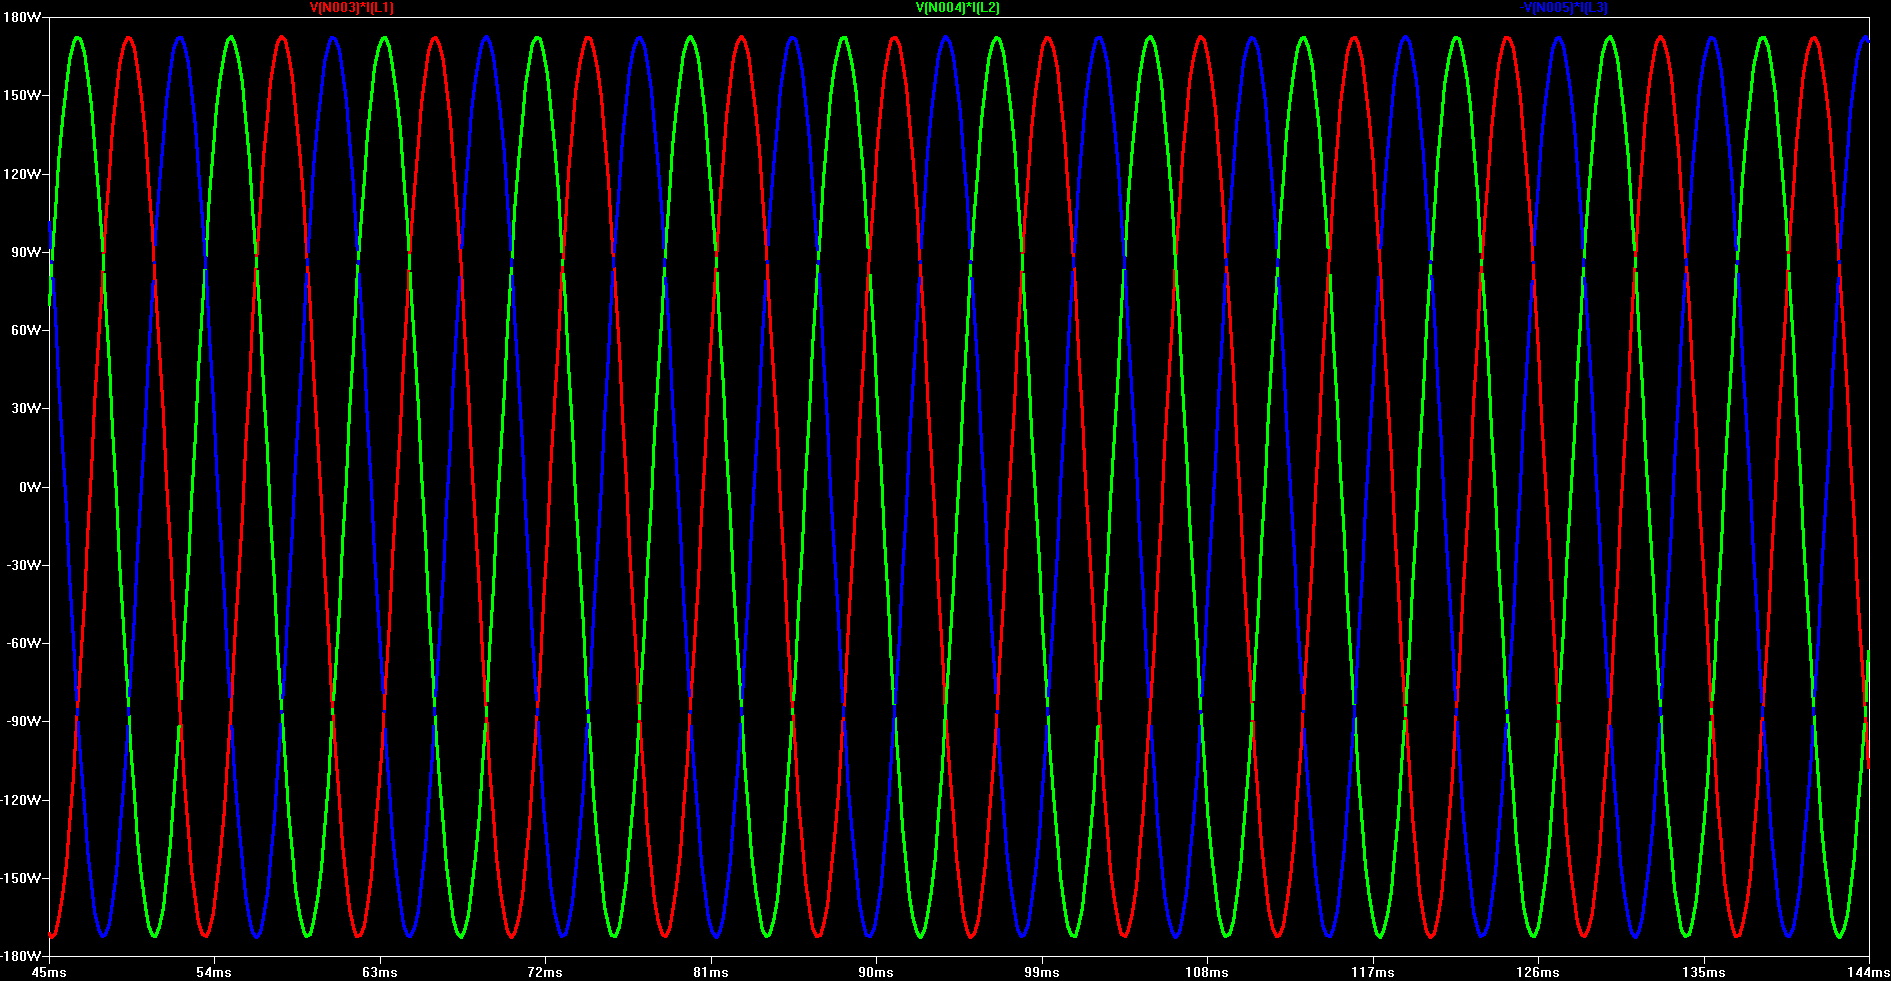
\includegraphics[width=\columnwidth]{images/Lab_9_ss_12.PNG}
    \captionof{figure}{Instantaneous power through the inductor}
    \label{fig:inst_power_inductor}
    \medskip
\endgroup

\begingroup
    \centering
    \medskip
    %width=\columnwidth
    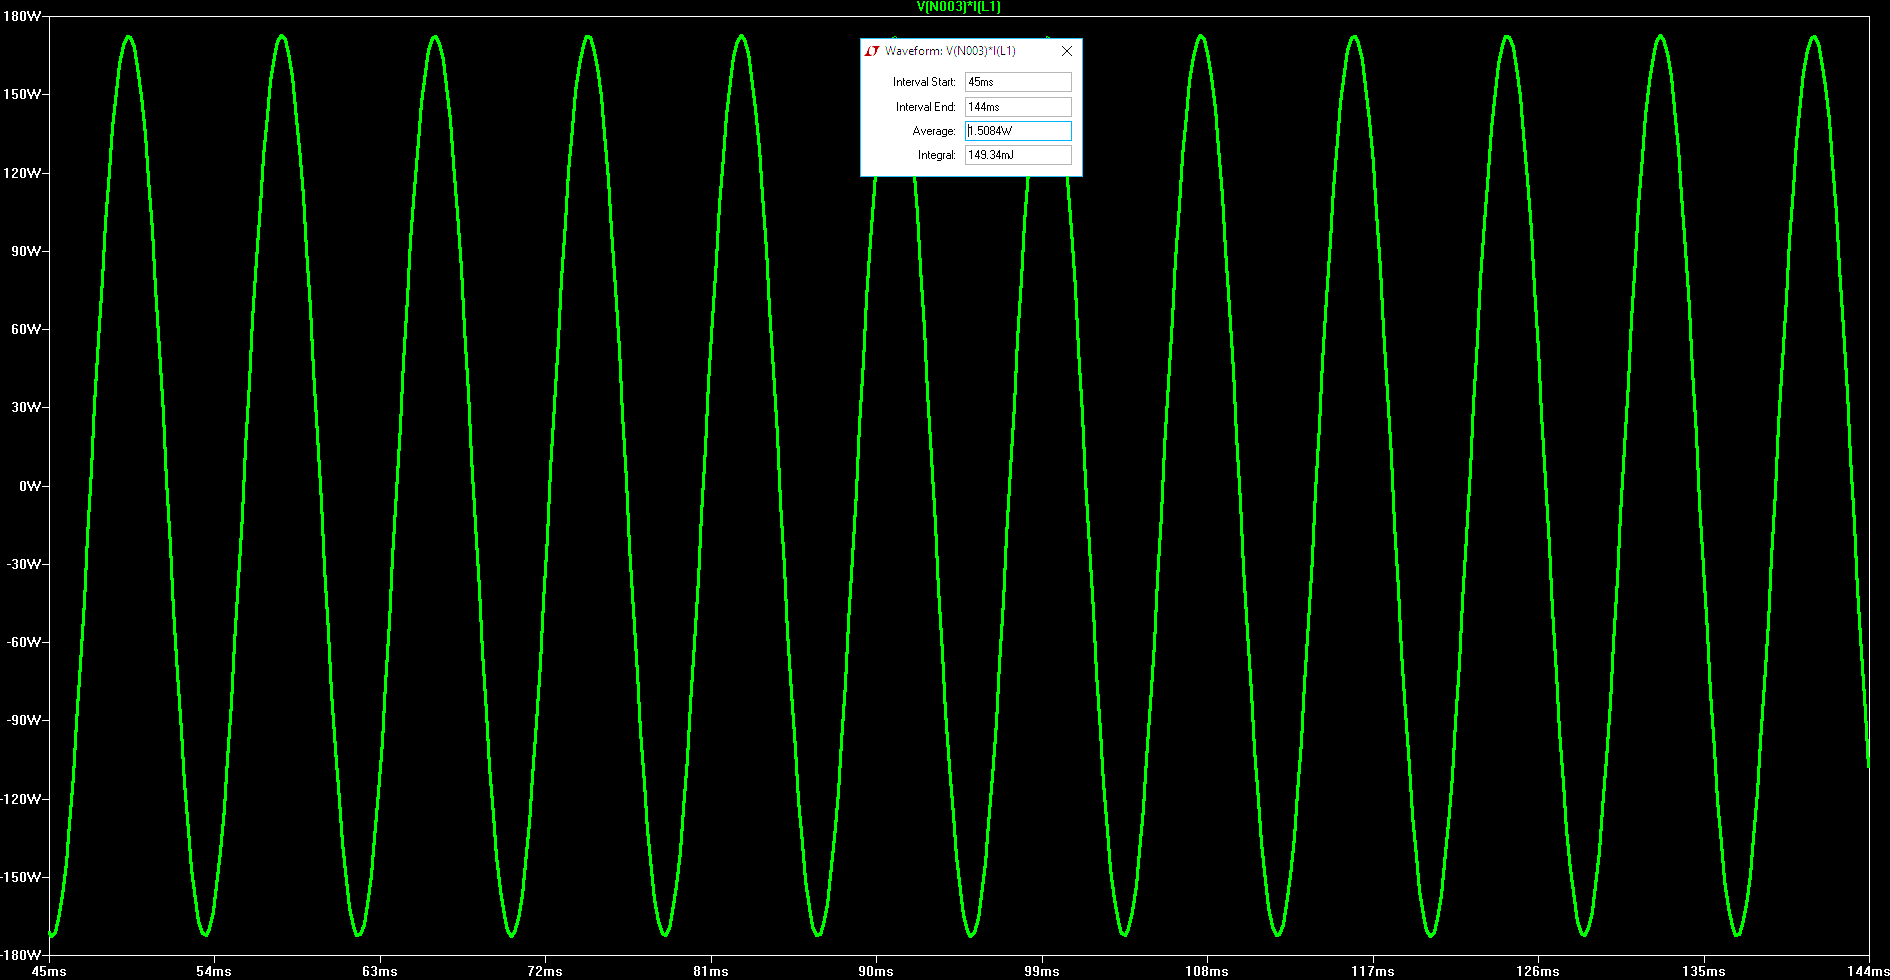
\includegraphics[width=\columnwidth]{images/Lab_9_ss_17.PNG}
    \captionof{figure}{Simulation value of the average power through the inductor}
    \label{fig:avg_power_inductor}
    \medskip
\endgroup

\noindent Equation \ref{eq:calc4} calculates the average power across the resistor.

\begin{equation} 
I^2 \cdot R = {2.00 \angle -59.99}^2 \cdot 50 = 100 \angle -59.99 W
\label{eq:calc4}
\end{equation}


\begingroup
    \centering
    \medskip
    %width=\columnwidth
    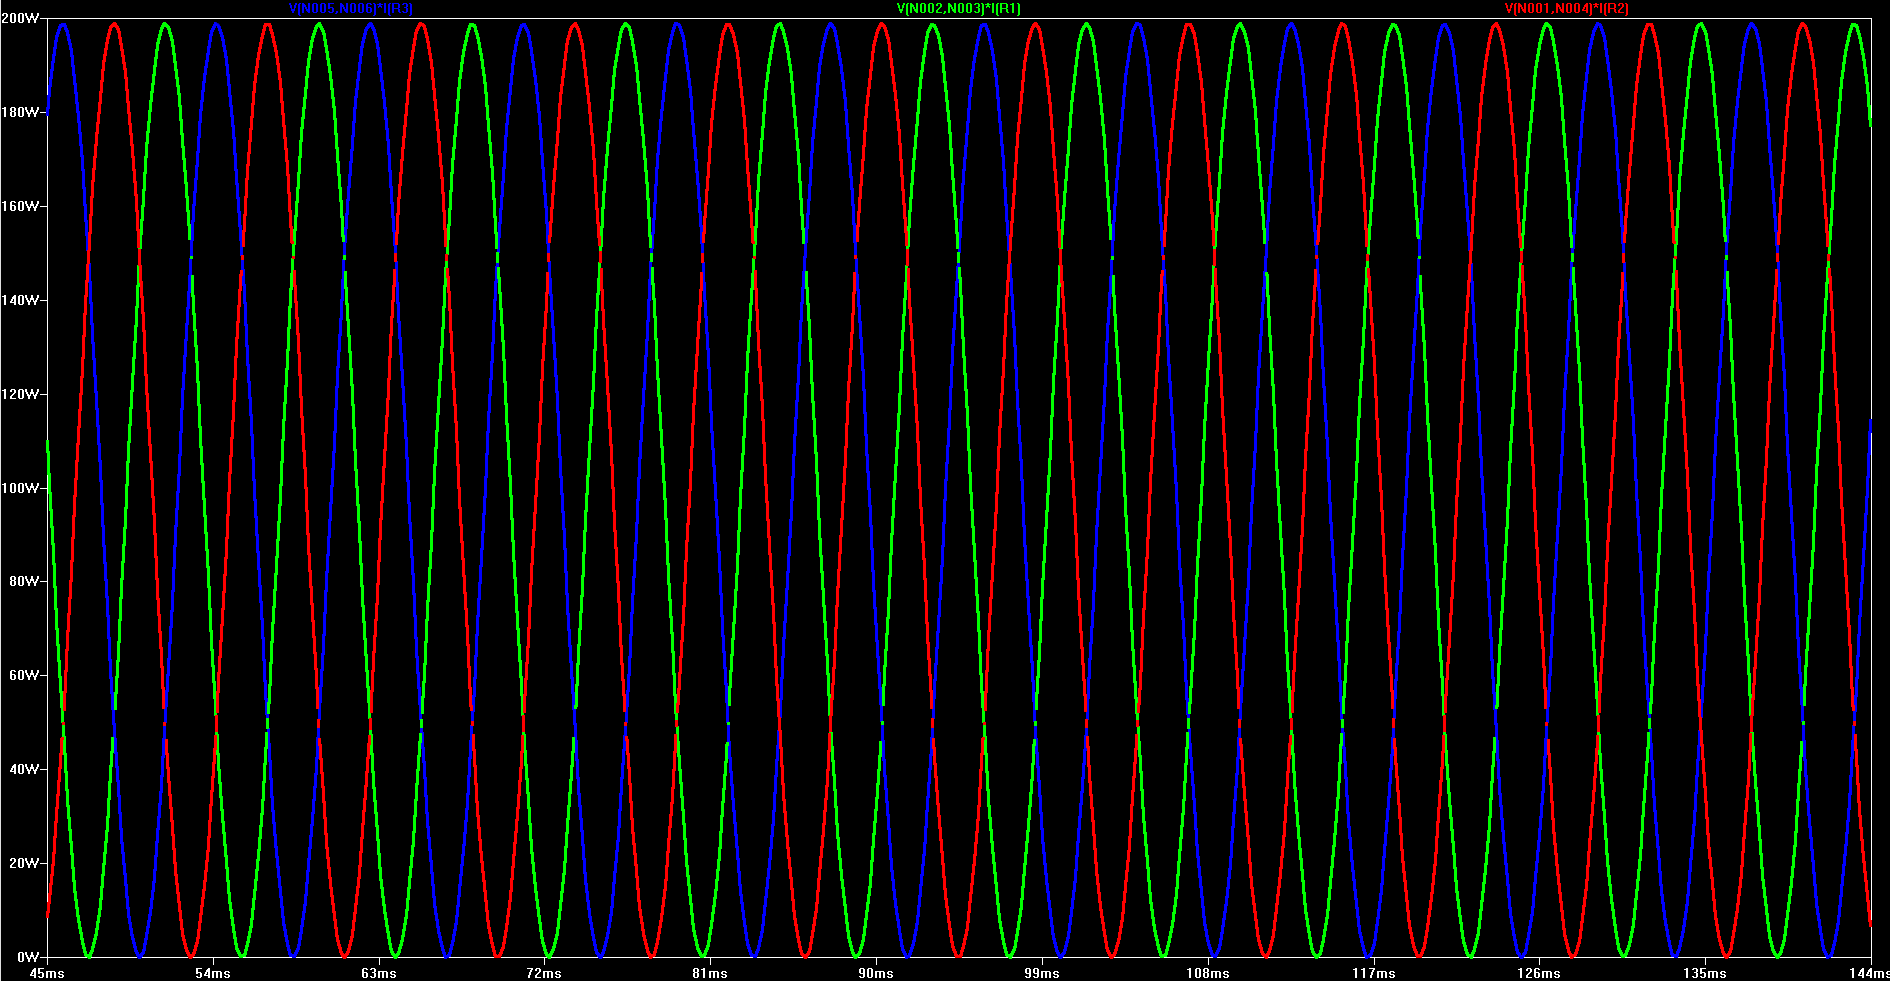
\includegraphics[width=\columnwidth]{images/Lab_9_ss_13.PNG}
    \captionof{figure}{Instantaneous power through the resistor}
    \label{fig:inst_power_rsistor}
    \medskip
\endgroup

\begingroup
    \centering
    \medskip
    %width=\columnwidth
    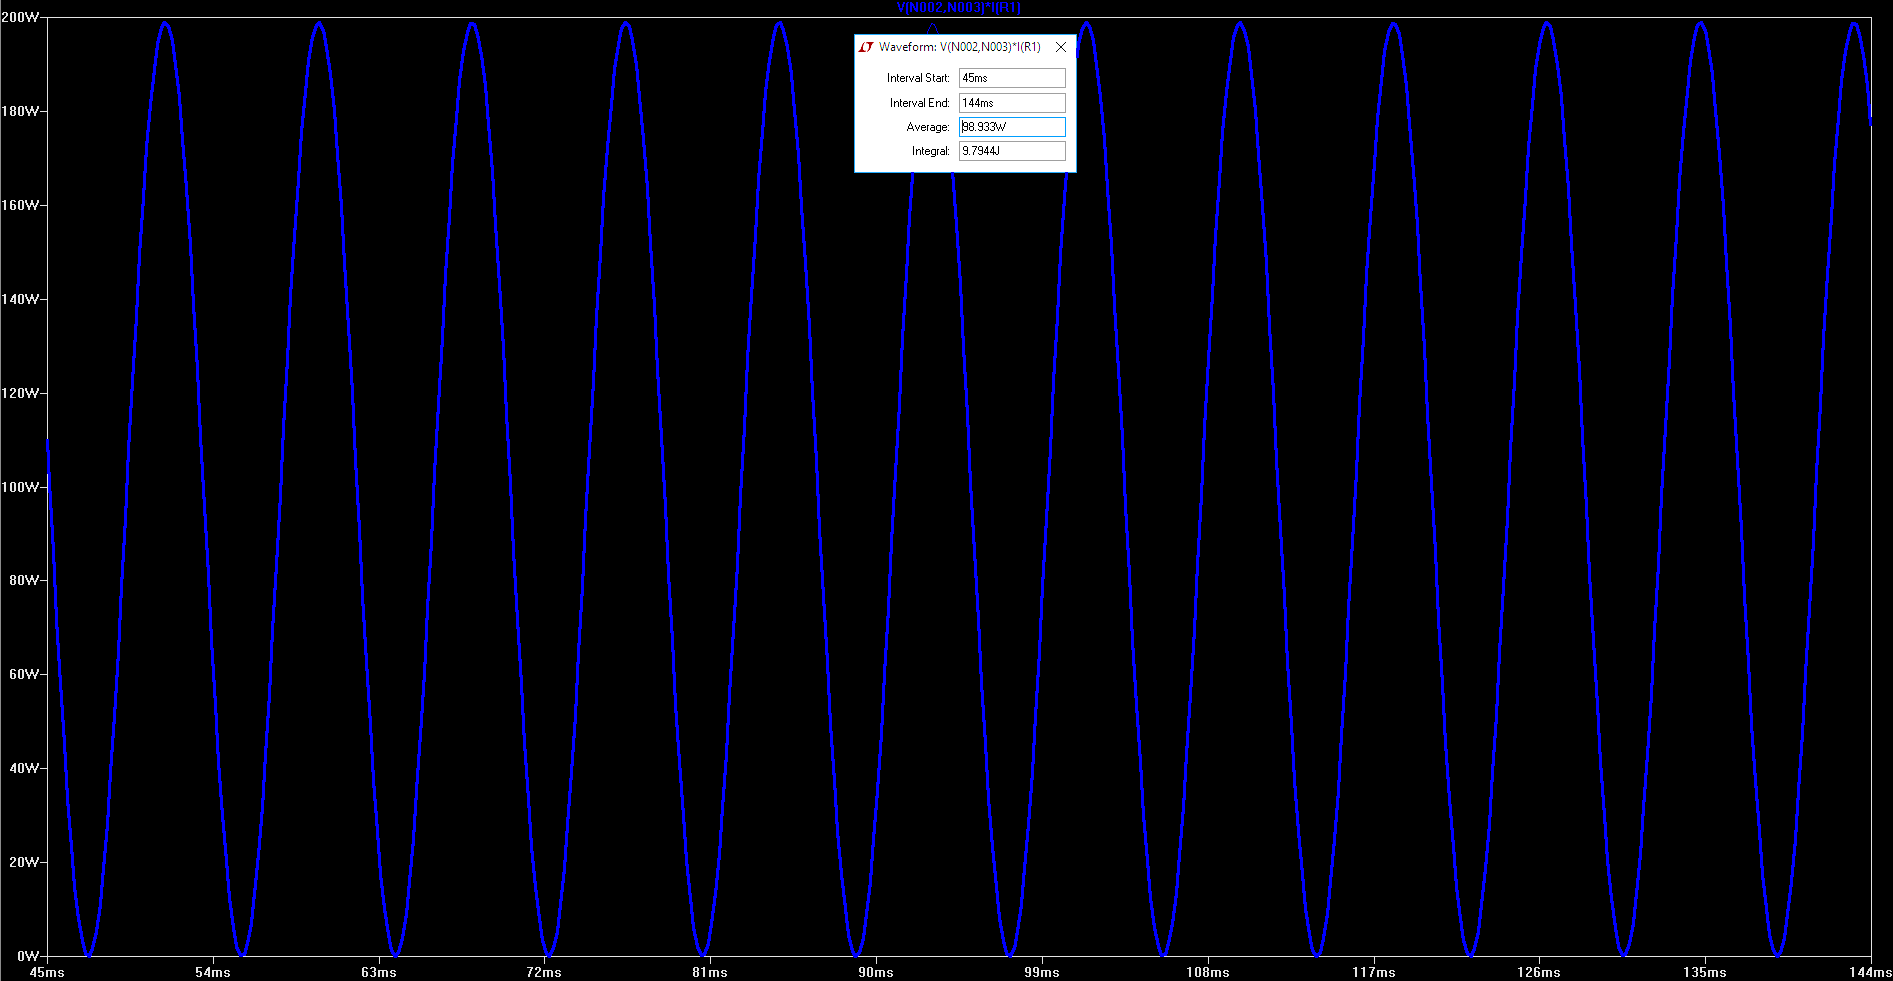
\includegraphics[width=\columnwidth]{images/Lab_9_ss_16.PNG}
    \captionof{figure}{Average power through the resistor}
    \label{fig:avg_power_resistor}
    \medskip
\endgroup


\noindent When the y-axes of Figures \ref{fig:avg_power_inductor} and  \ref{fig:avg_power_resistor} are closely analyzed, it is clear that the resistor has a range from 0W to 200W, while the inductor has a range from -180W to 180W. This situation shows that the resistor is a passive component and is able to dissipate power. On the contrary, the inductor both supplies and absorbs power, never truly dissipating power like the resistor. The simulation's choice to plot the inductor's power from a value of around -180W to 180W, results in an average power dissipation of approximately 1W, as seen in \ref{fig:avg_power_inductor}. This reflects the reality that inductors do not actually absorb any watt-power aside from minor heat loss. However, the resistor sees an average power of 100W, which accurately reflects the value obtained from equation \ref{eq:calc4}.

\noindent Analyzing the power through the power source shows a similar phenomena. According to equation \ref{eq:calc5}, the apparent power supplied to the circuit should be 400 VA. Looking at Figures \ref{fig:inst_power_power} and \ref{fig:avg_power_power}, we see that this value is reflected in the peak-peak value since the traces are plotted from -300 to 100. Interestingly, taking the average of this peak-peak value gives -100W, which is the expected real watt-power that is provided by the power source to the resistor.

\begin{equation} 
S = {2.00 \angle -59.99} \cdot 20 \angle 0 = 400 \angle -59.99 VA
\label{eq:calc5}
\end{equation}

\begingroup
    \centering
    \medskip
    %width=\columnwidth
    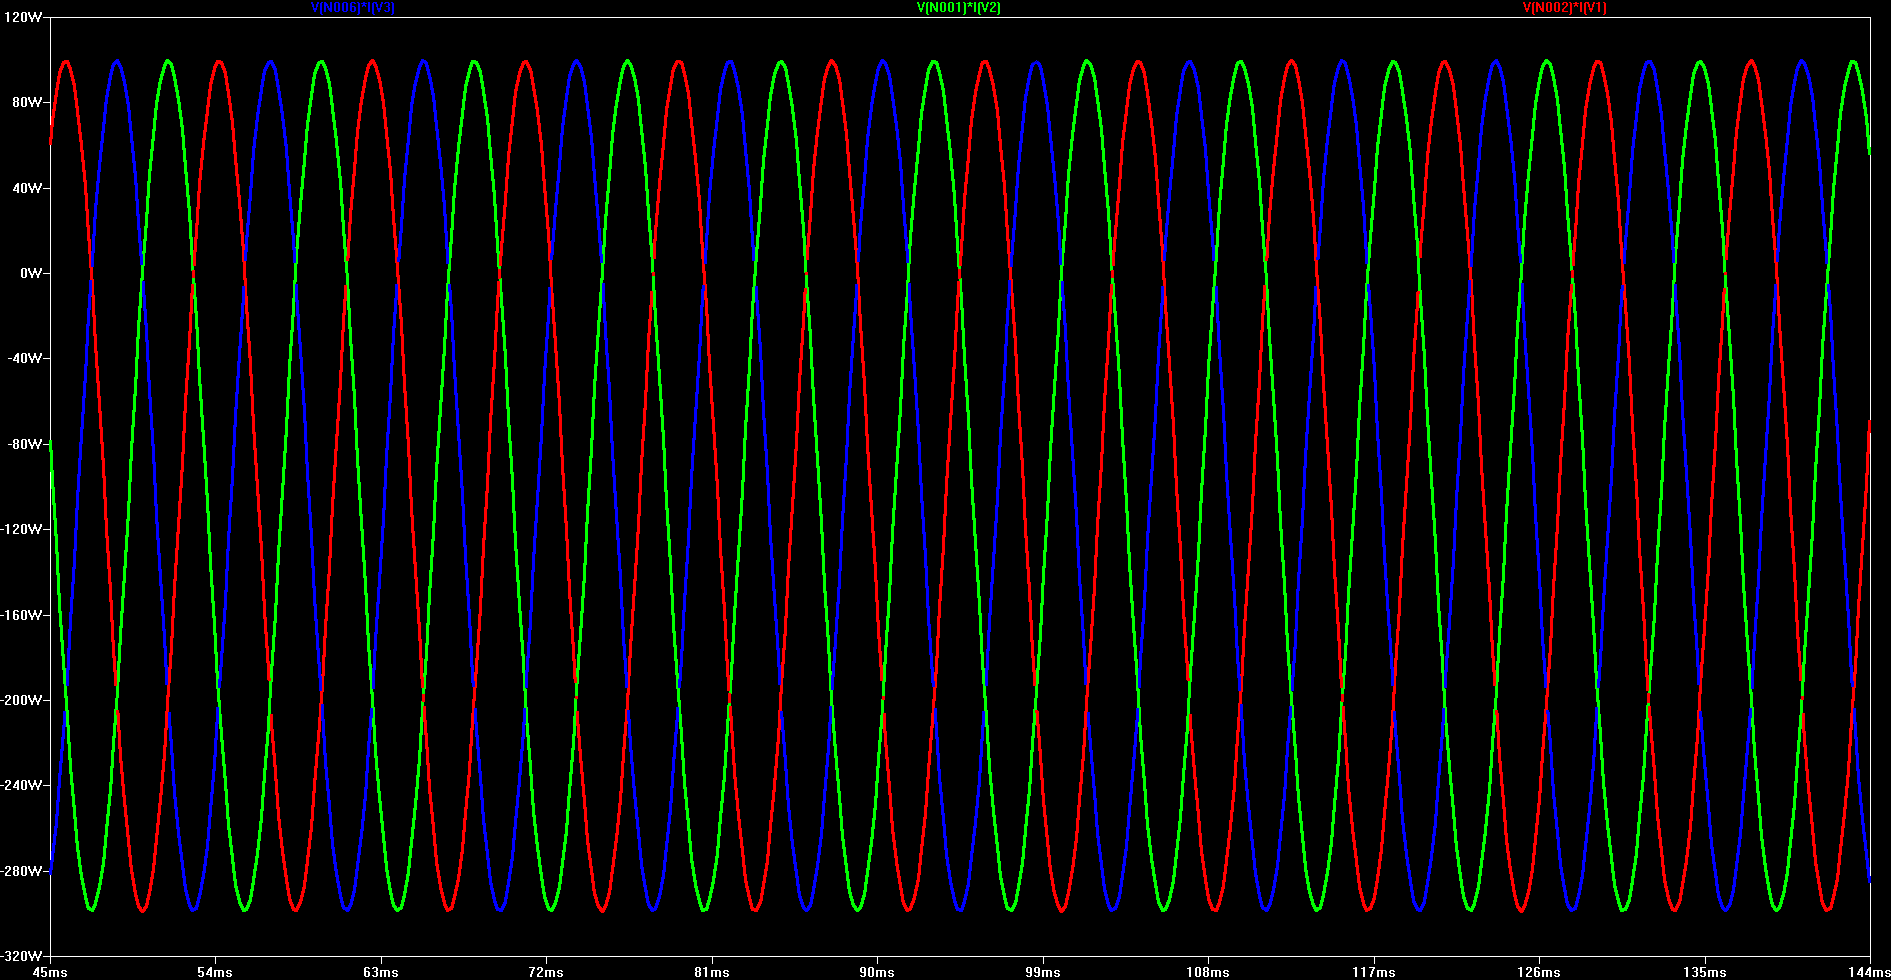
\includegraphics[width=\columnwidth]{images/Lab_9_ss_14.PNG}
    \captionof{figure}{  inst  power through power source}
    \label{fig:inst_power_power}
    \medskip
\endgroup


\begingroup
    \centering
    \medskip
    %width=\columnwidth
    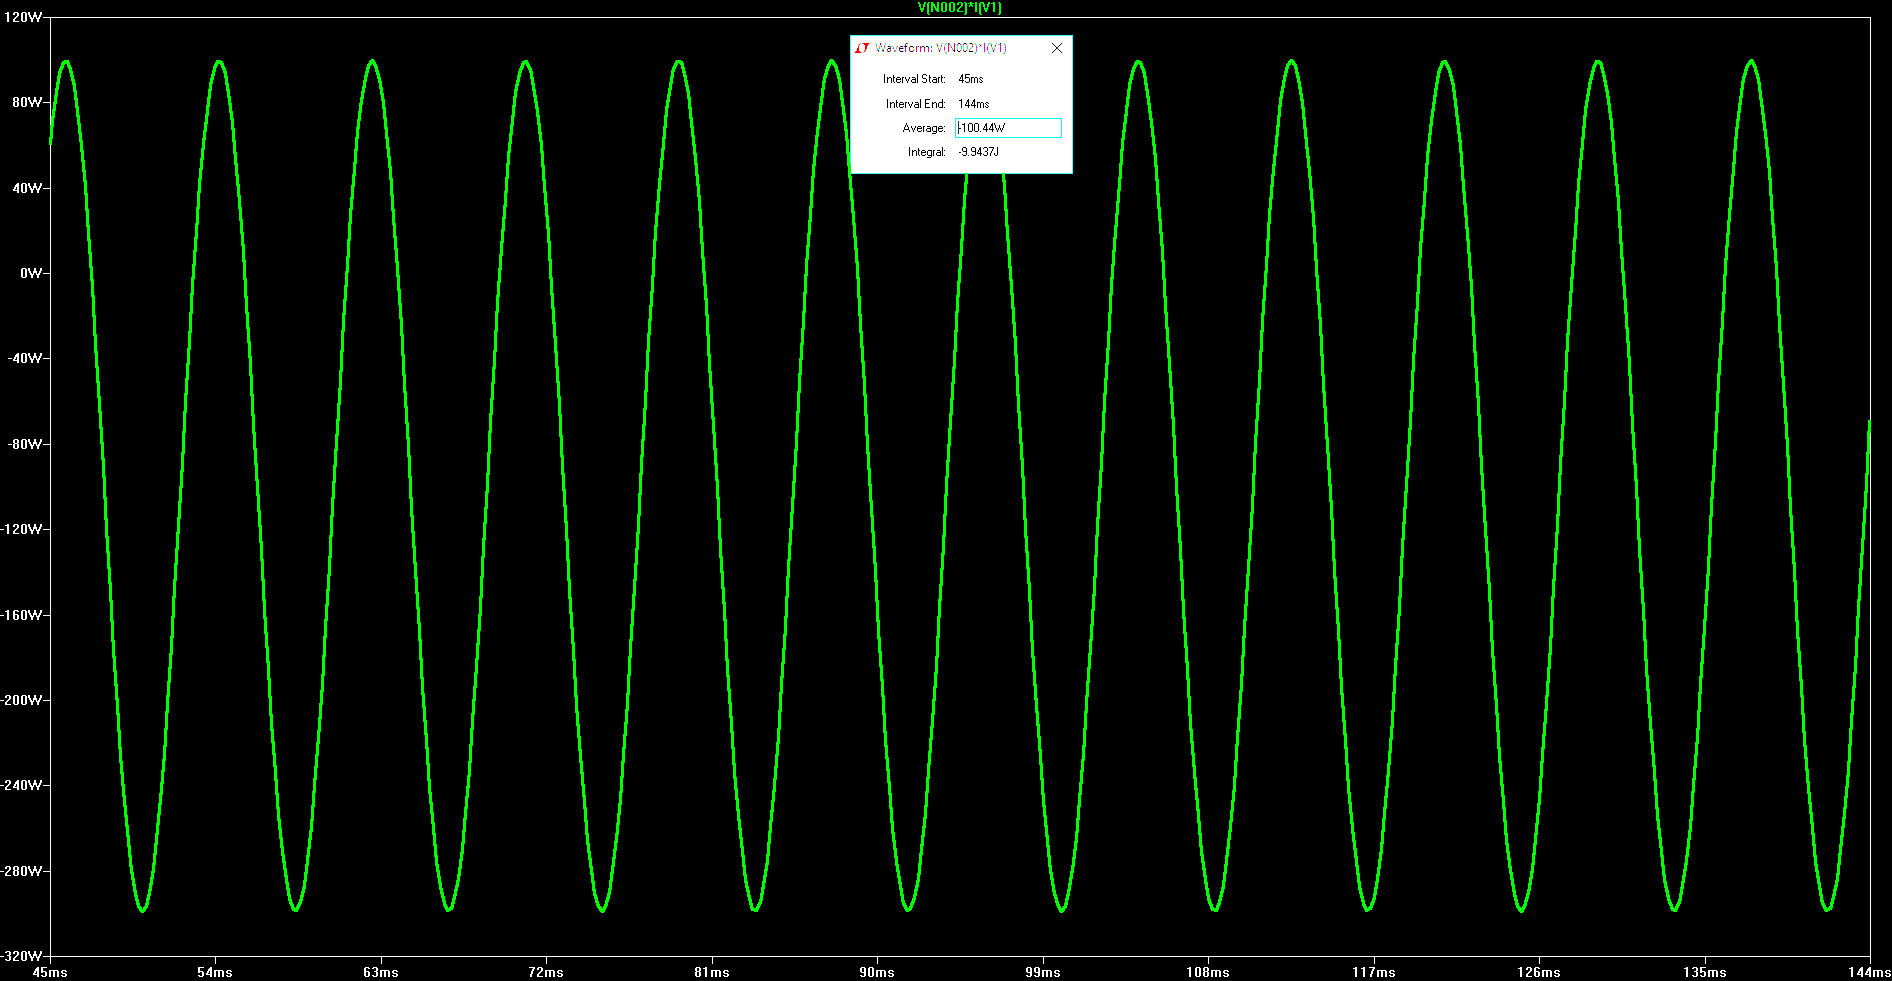
\includegraphics[width=\columnwidth]{images/Lab_9_ss_15.PNG}
    \captionof{figure}{  average power of power source}
    \label{fig:avg_power_power}
    \medskip
\endgroup

Hence, we see that the LTSpice software provides an interesting way of depicting imaginary and real power. In cases of imaginary power, it is reflected through the peak-peak value; moreover, the values are plotted in such a way that when taking the average, it results the real power that is dissipated through the component or circuit. 

%%%%%%%%%%%%%%%%%
%% Conclusions %%
%%%%%%%%%%%%%%%%%
\section{Conclusions}
% Understanding and applications

\noindent As a result of this experiment, we learned how instantaneous \& average power, line voltage \& current, and phase voltage \& current changes at different points of a 3 phase wye-wye circuit. We also learned how to use different available probes in LTSpice software for AC circuit analysis. After building practical circuits in the last lab session, we had a chance to analyze AC circuits under ideal conditions and ideal components in this lab session. We also confirmed the graphs obtained from the simulation with our manual calculations. In addition to the calculations, we also learned caveat of using LTSpice and circuit simulations in general. For example, initially we forgot to connect both of the neutral nodes to the ground. Using this configuration resulted in getting gibberish results in the plots. Later, we connected both of the neutrals and simulation worked as expected. We learned that common grounding is important for the software that it can assume same voltage levels for these points can solve the equations successfully to plot the graphs.  
\\
\noindent We learned how wye-wye connection is can tolerate imbalanced loads and keep running. The wye-wye circuit we worked in the LTSpice has many more usage cases beyond checking the voltage values in a simulator. Due to their reliability and higher efficiency under imbalance loads, they are considered as practical connection types and proffered by majority of the heavy industries.


\printbibliography

\end{document}